% Generated by Sphinx.
\def\sphinxdocclass{report}
\documentclass[letterpaper,10pt,english]{sphinxmanual}
\usepackage[utf8]{inputenc}
\DeclareUnicodeCharacter{00A0}{\nobreakspace}
\usepackage[T1]{fontenc}
\usepackage{babel}
\usepackage{times}
\usepackage[Bjarne]{fncychap}
\usepackage{longtable}
\usepackage{sphinx}


\title{WATER Documentation}
\date{June 16, 2010}
\release{1.0}
\author{Wu Lizong}
\newcommand{\sphinxlogo}{}
\renewcommand{\releasename}{Release}
\makeindex

\makeatletter
\def\PYG@reset{\let\PYG@it=\relax \let\PYG@bf=\relax%
    \let\PYG@ul=\relax \let\PYG@tc=\relax%
    \let\PYG@bc=\relax \let\PYG@ff=\relax}
\def\PYG@tok#1{\csname PYG@tok@#1\endcsname}
\def\PYG@toks#1+{\ifx\relax#1\empty\else%
    \PYG@tok{#1}\expandafter\PYG@toks\fi}
\def\PYG@do#1{\PYG@bc{\PYG@tc{\PYG@ul{%
    \PYG@it{\PYG@bf{\PYG@ff{#1}}}}}}}
\def\PYG#1#2{\PYG@reset\PYG@toks#1+\relax+\PYG@do{#2}}

\def\PYG@tok@gu{\let\PYG@bf=\textbf\def\PYG@tc##1{\textcolor[rgb]{0.50,0.00,0.50}{##1}}}
\def\PYG@tok@gt{\def\PYG@tc##1{\textcolor[rgb]{0.00,0.25,0.82}{##1}}}
\def\PYG@tok@gs{\let\PYG@bf=\textbf}
\def\PYG@tok@gr{\def\PYG@tc##1{\textcolor[rgb]{1.00,0.00,0.00}{##1}}}
\def\PYG@tok@cm{\let\PYG@it=\textit\def\PYG@tc##1{\textcolor[rgb]{0.25,0.50,0.56}{##1}}}
\def\PYG@tok@vg{\def\PYG@tc##1{\textcolor[rgb]{0.73,0.38,0.84}{##1}}}
\def\PYG@tok@m{\def\PYG@tc##1{\textcolor[rgb]{0.13,0.50,0.31}{##1}}}
\def\PYG@tok@mh{\def\PYG@tc##1{\textcolor[rgb]{0.13,0.50,0.31}{##1}}}
\def\PYG@tok@go{\def\PYG@tc##1{\textcolor[rgb]{0.19,0.19,0.19}{##1}}}
\def\PYG@tok@ge{\let\PYG@it=\textit}
\def\PYG@tok@gd{\def\PYG@tc##1{\textcolor[rgb]{0.63,0.00,0.00}{##1}}}
\def\PYG@tok@il{\def\PYG@tc##1{\textcolor[rgb]{0.13,0.50,0.31}{##1}}}
\def\PYG@tok@cs{\def\PYG@tc##1{\textcolor[rgb]{0.25,0.50,0.56}{##1}}\def\PYG@bc##1{\colorbox[rgb]{1.00,0.94,0.94}{##1}}}
\def\PYG@tok@cp{\def\PYG@tc##1{\textcolor[rgb]{0.00,0.44,0.13}{##1}}}
\def\PYG@tok@gi{\def\PYG@tc##1{\textcolor[rgb]{0.00,0.63,0.00}{##1}}}
\def\PYG@tok@gh{\let\PYG@bf=\textbf\def\PYG@tc##1{\textcolor[rgb]{0.00,0.00,0.50}{##1}}}
\def\PYG@tok@ni{\let\PYG@bf=\textbf\def\PYG@tc##1{\textcolor[rgb]{0.84,0.33,0.22}{##1}}}
\def\PYG@tok@nl{\let\PYG@bf=\textbf\def\PYG@tc##1{\textcolor[rgb]{0.00,0.13,0.44}{##1}}}
\def\PYG@tok@nn{\let\PYG@bf=\textbf\def\PYG@tc##1{\textcolor[rgb]{0.05,0.52,0.71}{##1}}}
\def\PYG@tok@no{\def\PYG@tc##1{\textcolor[rgb]{0.38,0.68,0.84}{##1}}}
\def\PYG@tok@na{\def\PYG@tc##1{\textcolor[rgb]{0.25,0.44,0.63}{##1}}}
\def\PYG@tok@nb{\def\PYG@tc##1{\textcolor[rgb]{0.00,0.44,0.13}{##1}}}
\def\PYG@tok@nc{\let\PYG@bf=\textbf\def\PYG@tc##1{\textcolor[rgb]{0.05,0.52,0.71}{##1}}}
\def\PYG@tok@nd{\let\PYG@bf=\textbf\def\PYG@tc##1{\textcolor[rgb]{0.33,0.33,0.33}{##1}}}
\def\PYG@tok@ne{\def\PYG@tc##1{\textcolor[rgb]{0.00,0.44,0.13}{##1}}}
\def\PYG@tok@nf{\def\PYG@tc##1{\textcolor[rgb]{0.02,0.16,0.49}{##1}}}
\def\PYG@tok@si{\let\PYG@it=\textit\def\PYG@tc##1{\textcolor[rgb]{0.44,0.63,0.82}{##1}}}
\def\PYG@tok@s2{\def\PYG@tc##1{\textcolor[rgb]{0.25,0.44,0.63}{##1}}}
\def\PYG@tok@vi{\def\PYG@tc##1{\textcolor[rgb]{0.73,0.38,0.84}{##1}}}
\def\PYG@tok@nt{\let\PYG@bf=\textbf\def\PYG@tc##1{\textcolor[rgb]{0.02,0.16,0.45}{##1}}}
\def\PYG@tok@nv{\def\PYG@tc##1{\textcolor[rgb]{0.73,0.38,0.84}{##1}}}
\def\PYG@tok@s1{\def\PYG@tc##1{\textcolor[rgb]{0.25,0.44,0.63}{##1}}}
\def\PYG@tok@vc{\def\PYG@tc##1{\textcolor[rgb]{0.73,0.38,0.84}{##1}}}
\def\PYG@tok@sh{\def\PYG@tc##1{\textcolor[rgb]{0.25,0.44,0.63}{##1}}}
\def\PYG@tok@ow{\let\PYG@bf=\textbf\def\PYG@tc##1{\textcolor[rgb]{0.00,0.44,0.13}{##1}}}
\def\PYG@tok@mf{\def\PYG@tc##1{\textcolor[rgb]{0.13,0.50,0.31}{##1}}}
\def\PYG@tok@bp{\def\PYG@tc##1{\textcolor[rgb]{0.00,0.44,0.13}{##1}}}
\def\PYG@tok@c1{\let\PYG@it=\textit\def\PYG@tc##1{\textcolor[rgb]{0.25,0.50,0.56}{##1}}}
\def\PYG@tok@kc{\let\PYG@bf=\textbf\def\PYG@tc##1{\textcolor[rgb]{0.00,0.44,0.13}{##1}}}
\def\PYG@tok@c{\let\PYG@it=\textit\def\PYG@tc##1{\textcolor[rgb]{0.25,0.50,0.56}{##1}}}
\def\PYG@tok@sx{\def\PYG@tc##1{\textcolor[rgb]{0.78,0.36,0.04}{##1}}}
\def\PYG@tok@err{\def\PYG@bc##1{\fcolorbox[rgb]{1.00,0.00,0.00}{1,1,1}{##1}}}
\def\PYG@tok@kd{\let\PYG@bf=\textbf\def\PYG@tc##1{\textcolor[rgb]{0.00,0.44,0.13}{##1}}}
\def\PYG@tok@ss{\def\PYG@tc##1{\textcolor[rgb]{0.32,0.47,0.09}{##1}}}
\def\PYG@tok@sr{\def\PYG@tc##1{\textcolor[rgb]{0.14,0.33,0.53}{##1}}}
\def\PYG@tok@mo{\def\PYG@tc##1{\textcolor[rgb]{0.13,0.50,0.31}{##1}}}
\def\PYG@tok@kn{\let\PYG@bf=\textbf\def\PYG@tc##1{\textcolor[rgb]{0.00,0.44,0.13}{##1}}}
\def\PYG@tok@mi{\def\PYG@tc##1{\textcolor[rgb]{0.13,0.50,0.31}{##1}}}
\def\PYG@tok@gp{\let\PYG@bf=\textbf\def\PYG@tc##1{\textcolor[rgb]{0.78,0.36,0.04}{##1}}}
\def\PYG@tok@o{\def\PYG@tc##1{\textcolor[rgb]{0.40,0.40,0.40}{##1}}}
\def\PYG@tok@kr{\let\PYG@bf=\textbf\def\PYG@tc##1{\textcolor[rgb]{0.00,0.44,0.13}{##1}}}
\def\PYG@tok@s{\def\PYG@tc##1{\textcolor[rgb]{0.25,0.44,0.63}{##1}}}
\def\PYG@tok@kp{\def\PYG@tc##1{\textcolor[rgb]{0.00,0.44,0.13}{##1}}}
\def\PYG@tok@w{\def\PYG@tc##1{\textcolor[rgb]{0.73,0.73,0.73}{##1}}}
\def\PYG@tok@kt{\def\PYG@tc##1{\textcolor[rgb]{0.56,0.13,0.00}{##1}}}
\def\PYG@tok@sc{\def\PYG@tc##1{\textcolor[rgb]{0.25,0.44,0.63}{##1}}}
\def\PYG@tok@sb{\def\PYG@tc##1{\textcolor[rgb]{0.25,0.44,0.63}{##1}}}
\def\PYG@tok@k{\let\PYG@bf=\textbf\def\PYG@tc##1{\textcolor[rgb]{0.00,0.44,0.13}{##1}}}
\def\PYG@tok@se{\let\PYG@bf=\textbf\def\PYG@tc##1{\textcolor[rgb]{0.25,0.44,0.63}{##1}}}
\def\PYG@tok@sd{\let\PYG@it=\textit\def\PYG@tc##1{\textcolor[rgb]{0.25,0.44,0.63}{##1}}}

\def\PYGZbs{\char`\\}
\def\PYGZus{\char`\_}
\def\PYGZob{\char`\{}
\def\PYGZcb{\char`\}}
\def\PYGZca{\char`\^}
% for compatibility with earlier versions
\def\PYGZat{@}
\def\PYGZlb{[}
\def\PYGZrb{]}
\makeatother

\begin{document}

\maketitle
\tableofcontents
\phantomsection\label{index::doc}


目 录:


\chapter{前  言}
\label{foreword::doc}\label{foreword:foreword}\label{foreword:id1}
Todo


\chapter{科学目标与研究内容}
\label{water_aims:doc-aims}\label{water_aims::doc}\label{water_aims:id1}

\section{1.背景}
\label{water_aims:id2}
随着全球观测手段的出现和日趋成熟,以能量循环、水循环和生物化学循环为研究对象的地球表层系统科学已逐渐发展成为实验特征明显的科学。遥感对地观测系统的建立和应用,大大提高了地球表层系统科学研究的效率;各种物质和能量定量测试的新技术,也为这一学科的发展带来了新的契机 \footnote{
Zhen Du, Chen Shupeng. Progress and disciplinary frontiers of geographical research {[}J{]}. Advance in Earth Sciences, 2001, 16(5): 599-606. {[}郑度, 陈述彭. 地理学研究进展与前沿领域{[}J{]}. 地球科学进展, 2001, 16(5): 599-606.{]}
} 。科学工作者第一次可以从宏观到微观,从全球到区域,利用前所未有的先进手段观察地球表面的各种过程,并通过可重复的实验深入理解过程,进而发展定量描述这些过程的计算机模型。地球表层系统科学已成为实验科学!在地球表层系统科学从经验科学走向实验科学的进程中,一系列针对地表过程的大型观测试验扮演了重要的角色 \footnote{
Sellers PJ, Hall FG, Asrar G, et al. The First ISLSCP Field Experiment (FIFE) {[}J{]}. Bulletin of American Meteorological Society, 1988, 69(1): 22-27.
} \footnote{
Sellers P, Hall F, Margolis H, et al. The Boreal Ecosystem–Atmosphere Study (BOREAS): An overview and early results from the 1994 field year {[}J{]}. Bulletin of the American Meteorological Society, 1995, 76(9): 1549-1577.
} ,正是这些观测试验对地理学、水文学、生态学、大气科学和整个地球系统科学的快速发展起到了举足轻重的作用,许多试验甚至成为一个阶段科学认识和研究方法进步的里程碑。

在各类陆面过程试验中,寒区和干旱区也受到了高度的重视。在干旱区开展的典型试验包括撒哈拉沙漠南缘地区萨赫勒水文大气引导试验(HAPEX) \footnote{
Goutorbe JP, Lebel T, Tinga A, et al. HAPEX-SAHEL - A large-scale study of land-atmosphere interactions in the semiarid tropics {[}J{]}. Annales Geophysicae, 1994, 12(1): 53-64.
} 以及我国科学家主导的黑河试验(HEIFE) \footnote{
Hu Yinqiao, Gao Youxi, Wang Jiemin, et al. Some achievements in scientific research during HEIFE {[}J{]}. Plateau Meteorology, 1994, 13(3): 225-236. {[}胡隐樵, 高由禧, 王介民, 等. 黑河实验(HEIFE)的一些研究成果{[}J{]}. 高原气象, 1994, 13(3): 225-236.{]}
}  \footnote{
Wang Jiemin. Land surface process experiments and interaction study in China – from HEIFE to IMGRASS and GAME-Tibet/TIPEX {[}J{]}. Plateau Meteorology, 1999, 18(3): 280-294. {[}王介民. 陆面过程实验和地气相互作用研究――从HEIFE到IMGRASS 和GAME-Tibet/ TIPEX{[}J{]}. 高原气象, 1999, 18(3): 280-294.{]}
} 、内蒙古半干旱草原土壤-植被-大气相互作用试验(IMGRASS) \footnote{
Lu Daren, Chen Zuozhong, Wang Genchen, et al. Inner Mongolia semi-arid grassland soil-vegetation-atmosphere interaction {[}J{]}. Climatic and Environmental Research, 1997, 2(3): 199-209. {[}吕达仁, 陈佐忠, 王庚辰, 等. 内蒙古半干旱草原土壤-植被-大气相互作用――科学问题与实验计划概述{[}J{]}. 气候与环境研究, 1997, 2(3): 199-209.{]}
} \footnote{
Lu Daren, Chen Zuozhong, Chen Jiayi, et al. Study on soil-vegetation-atmosphere interaction in Inner-Mongolia semi-arid grassland {[}J{]}. ACTA Meteorologica Sinica, 2005, 63(5): 571-593. {[}吕达仁, 陈佐忠, 陈家宜, 等. 内蒙古半干旱草原土壤-植被-大气相互作用综合研究{[}J{]}. 气象学报, 2005, 63(5): 571-593.{]}
} 、西北干旱区陆-气相互作用试验(NWC-ALIEX) \footnote{
Zhang Qiang, Huang Ronghui, Wang Sheng, et al. NWC-ALIEX and its research advances {[}J{]}. Advance in Earth Sciences, 2005, 20(4): 427-441. {[}张强, 黄荣辉, 王胜, 等. 西北干旱区陆-气相互作用试验NWC-ALIEX及其研究进展{[}J{]}. 地球科学进展, 2005, 20(4): 427-441.{]}
} 。这几个试验的特点都是从陆气相互作用着手,侧重于对大气边界层的观测,其目的是为大气模式中的陆面参数化服务,对于各个尺度上水文和生态过程的观测则相对较为薄弱。寒区由于观测条件困难,近年来才在气候与冰冻圈研究(CliC)等科学计划的催生下,得以有寒区陆面过程试验(CLPX) \footnote{
Cline D, Davis RE, Edelstein W, et al. Cold Land Processed Field Experiment Plan {[}R{]}. 1999.
} 的实施。CLPX强调对雪和冻土状态的观测,但忽视了它们的水文过程。因此,寒区和干旱区的陆面过程试验――特别是以理解和模拟各种尺度的水文与生态过程为目标的综合试验还有待加强,而在其实施过程中,还应高度关注寒区和干旱区在地域上的相互交织以及在各种过程上的联系和相互作用。

中国西部地区有着鲜明的寒区和旱区相伴而生的特点,特别是内陆河流域,具有全球独特的以水为纽带的“冰雪/冻土-森林-河流-湖泊-绿洲-荒漠”多元自然景观,一般从河流的源头到尾闾顺次分布着高山冰雪带、草原森林带、平原绿洲带和戈壁荒漠带等自然地理单元,是在流域尺度上开展寒区和干旱区水文和生态等陆面过程研究的理想场所。近年来,以流域为基本单元,围绕水-土-气-生-人相互作用作用,国内科技界开展了一系列卓有成效的研究,并且逐渐认识到必须以现代地球系统科学的思想为指导,以现代模型模拟及信息获取与处理技术为手段,开展综合集成研究,才能更好地立足于科学前沿的探索,同时也服务于未来的国家需求 \footnote{
Cheng Guodong, Li Xin, Kang Ersi, et al. Integrated Model Development and Modeling Environment Building for Interdisciplinary Studies in the Heihe River Basin {[}R{]}. Lanzhou: Cold and Arid Regions Environmental and Engineering Research Institute, CAS, 2008. 352 pp. {[}程国栋, 李新, 康尔泗, 等. 黑河流域交叉集成研究的模型开发和模拟环境建设 {[}R{]}. 兰州: 中国科学院寒区旱区环境与工程研究所, 2008. 352 pp.{]}
} 。显然,集成研究中机理剖析的深入和综合模型的建立,无不有赖于高分辨率、高质量和系统化的基础数据集,但无论是现有的观测数据或者是国际上其他地区的陆面过程试验数据,都无法满足流域科学集成研究的要求,数据瓶颈的问题十分突出。因此,亟待开展一次基础性的、多尺度的、多学科联合的、精心设计的综合观测试验。这种综合观测试验是提高对寒区和干旱区水循环和生态过程的定量化认识水平的基础。例如:寒区水文中,降水的观测和估计误差都很大,对冻土水文过程的认识甚为薄弱,对冰川和积雪的产流贡献也不清楚 \footnote{
Kang Ersi, Cheng Guodong, Dong Zengchuan. Glacier-Snow Water Resources and Mountain Runoff in the Arid Area of Northwest China {[}M{]}. Beijing: Science Press, 2002. pp 304. {[}康尔泗, 程国栋, 董增川. 中国西北干旱区冰雪水资源与出山径流{[}M{]}. 北京: 科学出版社, 2002. 304 pp.{]}
} 。干旱区水文研究中突出的问题包括:降水的高度异质性如何观测和模拟?地表水和地下水相互作用的过程是怎样的?内陆河流域尺度上的水分内循环是否存在,其量值有多大 \footnote{
Wheater HS, Sorooshian S, Sharma KD. Hydrological Modelling for Arid and Semi-Arid Areas {[}M{]}. Cambridge:  Cambridge University Press, 2008. 206 pp.
} ?自然和人为两种因素是如何相互作用而影响水文过程的 \footnote{
Wang Hao, Ruan Benqing, Shen Dajun. Water Price Theories and Practices for Sustainable Development {[}M{]}. Beijing: Science Press, 2003. 278 pp. {[}王浩, 阮本清, 沈大军. 面向可持续发展的水价理论与实践{[}M{]}. 北京: 清华大学出版社, 2003. 278 pp.{]}
} ?要解答这些问题,有赖于基础观测资料的积累,而遥感、同位素以及新一代的水文和生态观测手段,正在形成从地下到地表再到冠层、从微观到宏观的立体观测,为发展、改进和验证水文和生态等陆面过程模型提供着基础数据。开展流域综合观测试验,也是发展流域科学的重要前提。多年来,流域科学中的一些核心问题,如内陆河流域水资源的形成和转化规律以及水土资源的合理利用一直是国内科学界和决策部门关注的焦点问题之一。解决这些问题,有赖于利用现代计算机模拟技术以及广泛可获取的卫星遥感数据和其它空间数据,发展从整体上模拟流域过程和行为的流域集成模型。数据依然是前提!为此,发达国家提出了建立流域信息基础设施的构想,美国国家自然科学基金委员会计划在美国6个流域率先建立全自动化的观测网和先进的信息系统,以期给水科学和水管理带来革命性的变革 \footnote{
Atkins DE, Droegemeier KK, Feldman SI, et al. Revolutionizing Science and Engineering Through Cyberinfrastructure: Report of the National Science Foundation {[}R{]}. NSF, 2003.
} \footnote{
Neuse Prototype Hydrologic Observatory Design Team. Designing Hydrologic Observatories: A Paper Prototype of the Neuse Watershed {[}R{]}. Draft Version 4.0, 2004.
} 。观测系统和模拟平台的建立,无疑将是实现流域水资源和其他资源的精细管理,定量评估自然环境变化和人类活动对流域的影响,从而更好地为流域可持续发展服务的前提。

“黑河流域遥感-地面观测同步试验与综合模拟平台建设” (项目编号:KZCX2-XB2-09),正是在这样的背景下,从“中国科学院西部行动计划二期”“考虑长远,引领发展”的指导思想出发,经过反复论证,于2007年年中正式启动的重点研究项目 \footnote{
Huang Tieqing, Zhao Tao, Feng Renguo, et al. Project arrangement and primal progress in the second phase of the CAS Action Plan for West Development {[}J{]}. Advance in Earth Sciences, 2007, 22(9): 888-895. {[}黄铁青, 赵涛, 冯仁国, 等. 中国科学院西部行动计划(二期)项目布局与初步进展{[}J{]}. 地球科学进展, 2007, 22(9): 888-895.{]}
} 。本文将介绍项目中航空和卫星遥感与地面观测同步试验的科学背景、科学问题、研究目标以及观测试验方案和观测系统布置。


\section{2.科学问题与目标}
\label{water_aims:id20}
黑河流域遥感-地面观测同步试验将重点和优先解决以下科学问题:
\begin{enumerate}
\item {} 
遥感在多大程度上可以提高我们对于寒区水文、森林水文和干旱区水文过程的认识?

\item {} 
如何通过尺度转换,将多源和多尺度的遥感与地面观测资料相结合,应用于水文、生态及流域集成模型?

\item {} 
如何在陆面数据同化系统中有效地融合多源卫星遥感观测,实现对流域水文和生态过程的动态监测?

\end{enumerate}

总体目标是:开展航空-卫星遥感与地面观测同步试验,为发展流域科学积累基础数据;发展能够融合多源遥感观测的流域尺度陆面数据同化系统,为实现卫星遥感对流域的动态监测提供方法和范例。

具体的观测试验目标是:
\begin{enumerate}
\item {} 
以具备鲜明的高寒与干旱区伴生为主要特征的黑河流域为试验区,以水循环为主要研究对象,利用航空遥感、卫星遥感、地面雷达、水文气象观测、通量观测、生态监测等相关设备,开展航空、卫星和地面配合的大型观测试验,精细观测干旱区内陆河流域高山冰雪和冻土带、山区水源涵养林带、中游人工绿洲及天然荒漠绿洲带的水循环和生态过程的各个分量。

\item {} 
以航空遥感为桥梁,通过高精度的真实性验证,发展尺度转换方法,改善从卫星遥感资料反演和间接估计水循环各分量及与之密切联系的生态和其他地表过程分量的模型和算法。

\item {} 
发展流域尺度的陆面/水文数据同化系统,集成观测与模拟结果,生成高分辨率的、时空一致性的高质量数据集;进一步发展能够实时融合多源遥感观测的数据同化系统,实现卫星遥感对流域水文与生态过程的动态监测。

\item {} 
建立一个开放的试验场所和一套完全共享的多尺度综合数据集。

\end{enumerate}


\section{3.试验观测内容}
\label{water_aims:id21}
黑河流域遥感-地面观测同步试验由三个试验,包括寒区水文试验、森林水文试验和干旱区水文试验,以及一个集成研究,即模拟平台和数据平台建设组成。


\subsection{3.1上游寒区水文试验}
\label{water_aims:id22}
在寒区水文试验区开展微波辐射计、激光雷达、高光谱航空遥感试验。利用机载多波段微波辐射计获取雪深、地表冻融状况和土壤水分;利用机载激光雷达测量雪深和地表粗糙度;从高光谱遥感提取雪盖面积、雪反射率、雪粒径及试验区地表覆盖类型。以航空遥感为桥梁、以地面真实性检验为标准,重点研究卫星数据反演雪水当量和土壤冻融的方法和精度。选择典型小流域同步开展双偏振多普勒雷达降水观测,地基微波辐射计观测,建立寒区水文径流场,加密观测寒区水文过程,定点测量积雪和冻土的各种物理属性和水热变化特征。获取同期的雷达、被动微波、可见光近红外和热红外卫星遥感数据,研究多尺度数据在空间和时间尺度上的转换机制。构建用于发展、改进和验证寒区陆面过程模型和分布式水文模型所需的数据集。


\subsection{3.2森林水文试验}
\label{water_aims:id23}
在森林水文试验区开展高光谱、多角度热红外、激光雷达航空遥感试验。从高光谱遥感提取生物物理参数及植被类型;利用多角度热红外遥感器,获取森林、灌丛和草地的观测数据,反演地表和冠层温度;利用激光雷达测量植被的三维结构,并估算生态系统生产力。利用以上观测/反演量提高对森林水文的重要分量――蒸散发、截留、树干径流、透过流的估算精度。获取同期的可见光近红外和热红外卫星遥感数据及雷达降雨观测数据。选择重点小流域加密观测森林水文和生态过程。构建用于发展、改进和验证森林水文模型和生态模型所需的数据集。


\subsection{3.3中游干旱区水文试验}
\label{water_aims:id24}
在干旱区水文试验区开展高光谱、多角度热红外、激光雷达、微波辐射计航空遥感试验。从高光谱遥感提取生物物理参数及地表覆盖类型;利用多角度热红外遥感资料反演地表和冠层温度;利用激光雷达测量植被的三维结构和粗糙度;利用微波辐射计观测土壤水分。获取同期的各类卫星遥感数据及雷达降雨观测数据。配合航空遥感试验开展地面同步观测试验。以临泽内陆河流域综合研究站和张掖国家气候观象台为依托,选择中游典型生态系统样带或样区,开展植被和土壤相关参数的地面加密观测试验。改善从航空遥感和卫星遥感资料反演和间接估计蒸散发的模型和算法,发展地面观测验证反演结果的尺度转换方案。


\subsection{3.4模拟平台和数据平台}
\label{water_aims:id25}
以现代陆面过程模型和水文水资源模型(包括地下水动态模型)为骨架,构建“大气-水文-生态”综合模拟模型平台。发展流域尺度的陆面/水文数据同化系统,集成观测与模拟结果,生成全流域空间分辨率为1km、时间分辨率为1小时的同化数据集。进一步发展能够实时融合多源遥感观测的数据同化系统,实现卫星遥感对流域水文与生态过程的动态监测。在“数字黑河”基础上,建立黑河遥感试验信息系统,发布原始试验数据、各级数据产品及同化数据。


\section{参考文献:}
\label{water_aims:id26}

\chapter{试验区介绍}
\label{water_experiment_area:water-experiment-area}\label{water_experiment_area::doc}\label{water_experiment_area:id1}
流域尺度的研究区选定为典型的内陆河流域――黑河流域,面积约12.87万km2,是我国第二大内陆河流域,位于东经96°42′~102°00′,北纬 37°41′~42°42′,包括高山冰雪带、森林草原带、平原绿洲带及戈壁荒漠带等不同的景观类型。黑河流域是我国内陆河流域研究的基地,具有良好的研究基础、完备的观测系统和丰富的数据积累。综合考虑内陆河流域的主要水文过程,包括寒区水文、森林水文、生态水文及干旱区水文,在全流域内,选择三个具有代表性的重点试验区开展综合观测试验。

综合考虑内陆河流域的主要水文过程,包括寒区水文、森林水文、生态水文及干旱区水文,“黑河流域遥感-地面观测同步试验”在全流域内,选择了三个具有代表性的重点试验区开展综合观测试验。

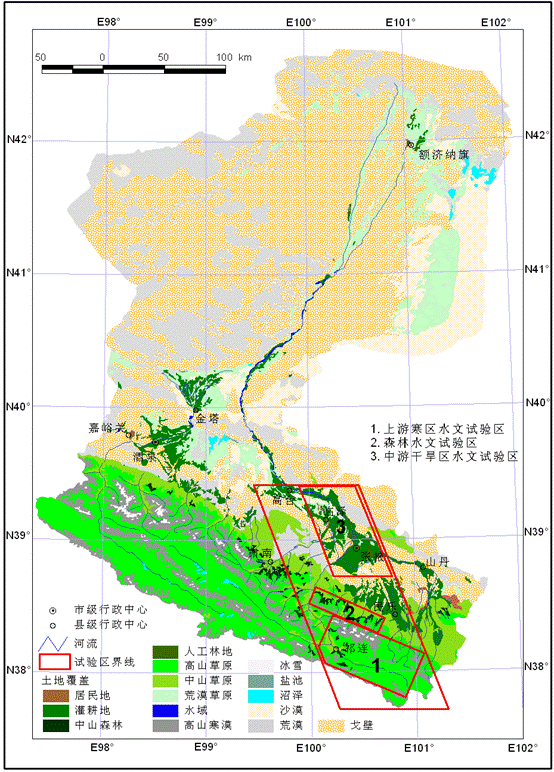
\includegraphics{experiment_heihe.png}

图1 黑河流域所处位置示意图


\section{1.上游寒区水文试验区}
\label{water_experiment_area:id2}
上游寒区水文试验区(Cold Region Hydrology Experiment Area)选择在黑河上游东侧(图3),面积约??平方公里,平均海拔高度。该区(请补充上游寒区水文实验区介绍性文字)。
上游寒区水文试验区包括重点试验区、加密观测区和观测点。重点试验区为黑河上游东支八宝河子流域。加密观测区选择冰沟小流域,开展降雨降雪观测,地面-遥感同步观测,以及寒区水文过程观测。观测点选择冰沟垭口、俄博岭垭口、野牛山头滩垭口、海潮坝、阿柔乡和扁都口,试验区布置见图3。

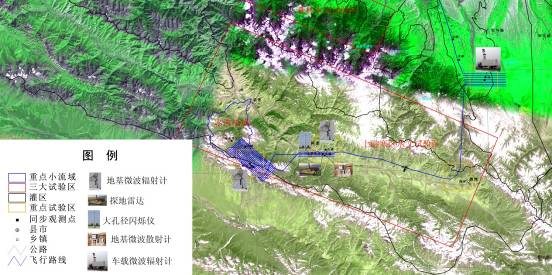
\includegraphics{cold_region.jpg}

图2 上游寒区水文试验区


\subsection{1.1 阿柔试验区}
\label{water_experiment_area:id3}
阿柔乡(100°26′N,38°03′E)位于八宝河流域中部河谷地带,海拔3000m,地势开阔平坦,交通便利,主要开展积雪和地表冻融状态的遥感-地面同步观测,并长期观测季节冻土的水热变化特征。


\subsection{1.2 冰沟试验区(Binggou)}
\label{water_experiment_area:binggou}
冰沟流域(38°01′~38°04′N,100°12′~100°18′E)位于黑河上游东支二级支流上(图5),海拔3450~4400m,平均为3920m。流域面积30.48km2,平均宽度3.59km,植被分布面积19.82km2,占流域总面积的65%左右。气象场年平均气温-2.5℃,最低气温-30.8℃,最高气温24.8℃,流域源头的年平均气温为-7℃。季节性积雪厚度约为0.5m,最深达0.8~1.0m。多年冻土下界可能在3400m左右。长期观测积雪、冻土、气象、植被等寒区水文变量与参数,并开展地基微波辐射计和野外光谱仪等项目综合观测。
补充历史上开展的积雪观测

图5 冰沟流域分布图


\subsection{1.3 扁都口试验区(Biandukou)}
\label{water_experiment_area:biandukou}
选择民乐县扁都口(100°56′N,38°13′E)以北平坦开阔地,平均海拔2800m,观测瞬时积雪参数及地表冻融状态,并与卫星过境同步,观测地表温度,验证被动微波地表冻融分类算法。


\section{2. 森林水文试验区}
\label{water_experiment_area:id4}
森林水文试验区(Forest Hydrology Experiment Area,简称FHEA),选择在黑河上游祁连山区(图6),面积约??km2,平均海拔。研究区内??(补充森林水文试验区介绍性文字)
选择大野口、海潮坝等一系列山前子流域,在景观类型上涵盖了冰川、积雪、多年冻土、高寒草原和森林。该试验区的主要观测对象为森林水文过程。

图6 森林水文和生态试验区位置图


\subsection{2.1 大野口流域(Dayekou Basin)}
\label{water_experiment_area:dayekou-basin}
大野口流域 (经纬度范围??)位于??,面积为100 km2,属高寒干旱半干旱气候(图7)。区内自然条件复杂,水热条件差异大,形成了多种具有明显垂直梯度和水平差异的植被类型和土壤类型。海拔从低到高,植被类型依次为山地荒漠植被、山地草原植被、山地森林草原植被、亚高山草甸植被、高山冰雪植被;土壤类型依次为山地灰钙土、山地栗钙土、山地灰褐土、亚高山灌丛草甸土、高山寒漠土。在各类土壤中山地灰褐土和亚高山灌丛草甸土是生长森林的土壤,山地灰褐土分布在海拔2400~3300 m地带,是乔木林的主要分布带;亚高山灌丛草甸土分布在海拔3300~4000 m 亚高山地带,是湿性灌木林的主要分布带。
研究区内现有水源林???hm2 ,主要为青海云杉林、祁连圆柏林和灌木三大类型。建群种青海云杉成块状分布在实验区海拔2400~3300 m 阴坡和半阴坡地带,与阳坡草场交错分布;祁连圆柏呈小块状分布于阳坡、半阳坡;灌木优势种有金露梅、箭叶锦鸡儿、吉拉柳等;草本主要有珠芽蓼、黑穗苔草等
研究区显著的垂直地带性分异规律以及分布广泛的青海云杉林和灌木林使其成为研究森林水文学的理想区域;并且甘肃省水源涵养林院在该流域内布设有系统的气象和水文观测系统,开展了大量生态样方调查,有研究基础和数据积累。

图7大野口流域及其地面观测系统


\section{3.干旱区水文试验区}
\label{water_experiment_area:id5}
干旱区水文试验区(Arid Region Hydrology Experiment Area)选择在黑河中游张掖、临泽和高台一带(图9)。该试验区内,以黑河干流莺落峡和正义峡两个水文站为地表水输入和输出控制点,形成一个完整的水循环系统。
试验区沿黑河主干流从张掖绿洲延伸到临泽和高台绿洲,是由人工绿洲生态系统、绿洲—荒漠过渡带生态系统、荒漠草原生态系统、荒漠生态系统和水域生态系统共同组成的荒漠绿洲景观系统。中游干旱区降水量一般小于200mm(由东南向西北减少),农业生产通过渠灌和井灌利用了流域内大量的水资源,是水资源耗用区域,主导着流域水循环和水文过程。

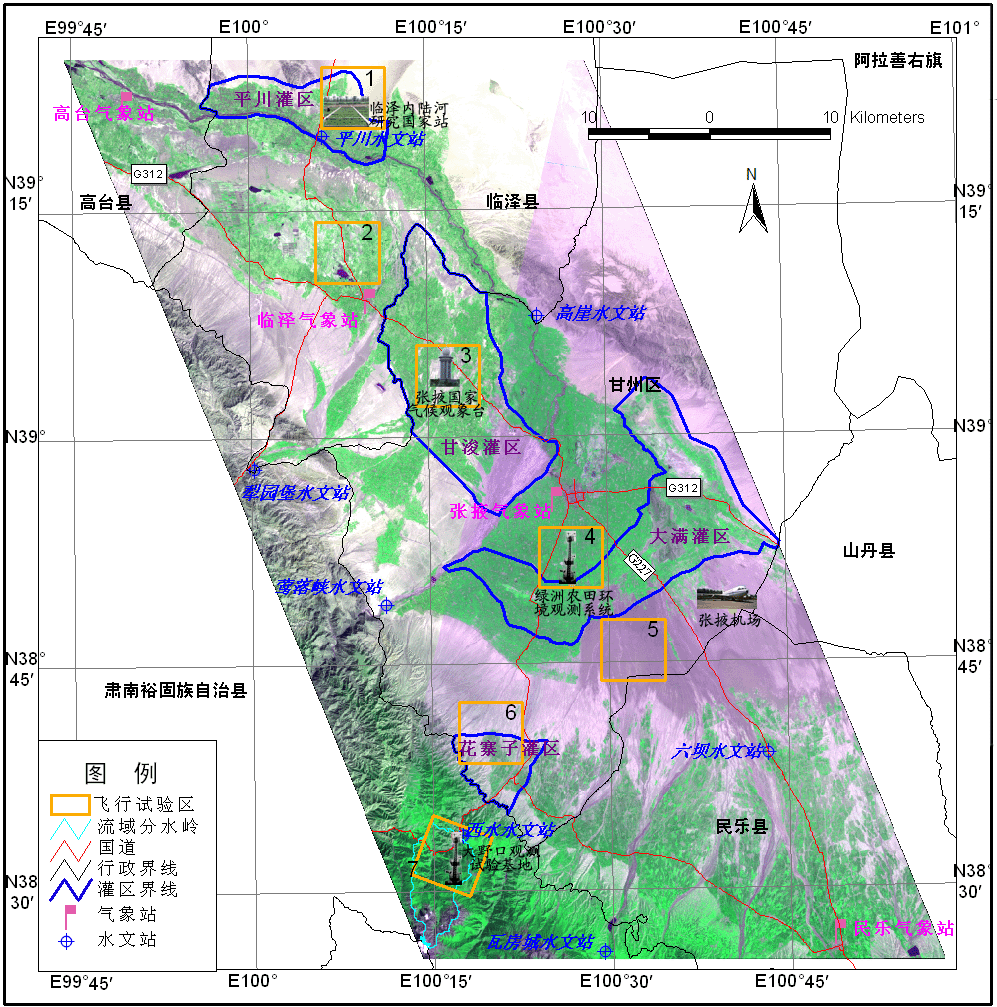
\includegraphics{arid_region.png}


\subsection{3.1 盈科绿洲观测站}
\label{water_experiment_area:id6}
图x 盈科草原观测区观测仪器布置图


\subsection{3.2 花寨子荒漠站}
\label{water_experiment_area:id7}
图x 临泽绿洲与荒漠过渡带观测站仪器布置图


\subsection{3.3 临泽国家站}
\label{water_experiment_area:id8}

\subsection{3.4 兰大草地站}
\label{water_experiment_area:id9}

\subsection{3.5 张掖城区观测站}
\label{water_experiment_area:id10}
图x 张掖城区观测站仪器布置图


\chapter{观测系统布置}
\label{water_observe_system:water-observe-system}\label{water_observe_system::doc}\label{water_observe_system:id1}

\section{1. 概述}
\label{water_observe_system:id2}
{\hfill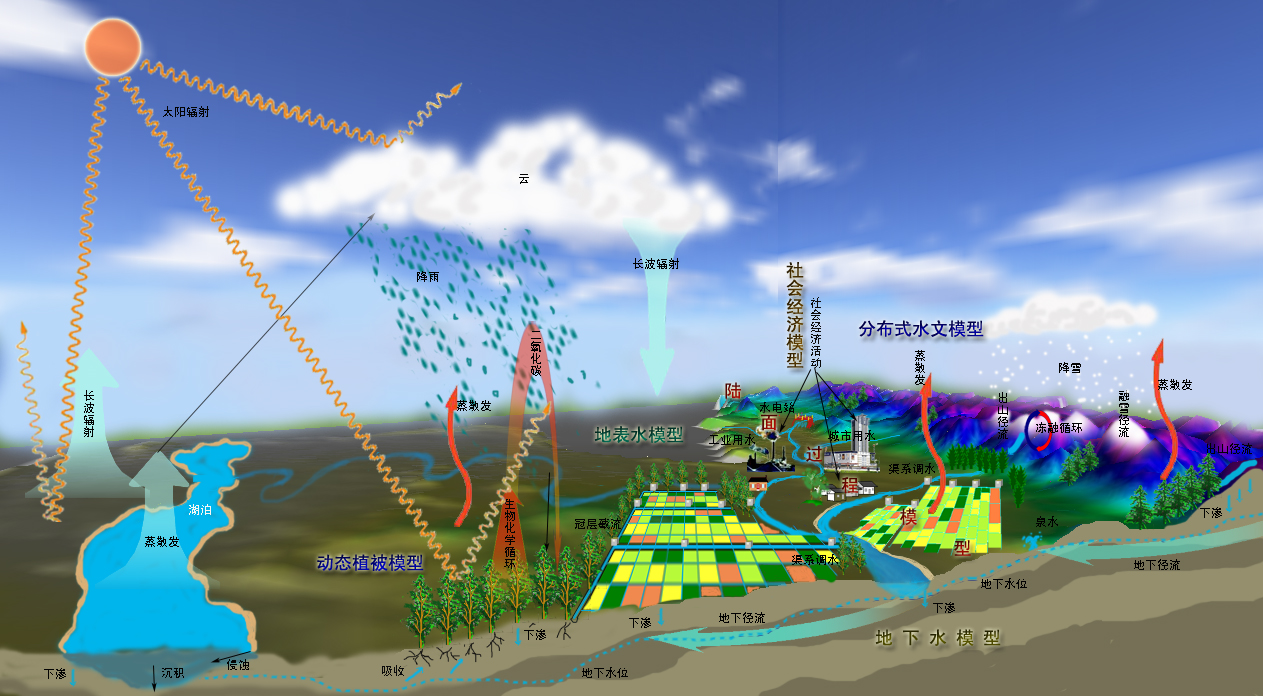
\includegraphics{observe_system.jpg}\hfill}

图1 黑河遥感观测试验概念图


\section{2. 通量和气象水文观测网络}
\label{water_observe_system:id3}
在黑河流域已有观测网络的基础上,黑河流域遥感-地面观测同步试验在三个重点试验区依据不同景观类型新建了7个自动气象站,4套涡动相关观测,2套大孔径闪烁仪。新建的观测系统和试验区已有的5个自动气象站,2套涡动相关,8个业务气象站及34个气象区域站相配合,在试验区(图 6)约23700 km2的范围内,形成了包括常规站(常规气象观测)、重点站(增加多层气象要素、辐射平衡4分量观测、多层土壤温度和土壤含水量以及浅层土壤热流观测)和重点加强站(增加湍流通量观测)三位一体的黑河中上游地区地面气象水文观测网,以满足不同层次研究和分析――特别是流域集成模型发展、改进和验证以及发展高分辨率驱动数据集的需要。试验区内通量和气象水文观测网络分布见图 6,表 6汇总了重点站和重点加强站的基本信息。

表X 通量和气象水文观测概念图

{\hfill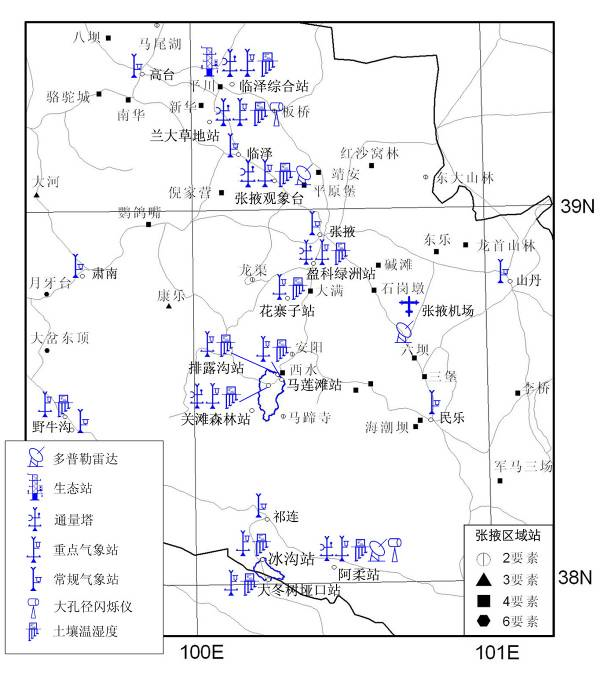
\includegraphics{metrology_system.png}\hfill}

图X黑河遥感试验常规气象观测系统
图 X  黑河遥感试验通量和气象水文观测网络
(区域站中,2要素是指气温和降水;3要素是指气温、降水和风向;4要素是指气温、降水、风向和风速;6要素是指气温、降水、风向、风速、气压和总辐射)

表X常规观测站
序号      站名      英文名称    唯一标识码   位置      观测项目    景观类型
1
2
3
4

表 X  气象水文重点站
序号      站名      英文名称    英文缩写或标识码        位置      观测项目    景观类型
1       阿柔冻融观测站                 100°27′E
38°03′N
3033 m  大气:风温湿梯度观测(2m \& 10m)、气压、降水;四分量辐射;地表热红外温度;土壤剖面:温度、水分、水势(10cm、20cm、40cm、80cm、120cm和160cm)及土壤热通量(5cm和15cm);涡动相关;大孔径闪烁仪     高山草原
2       冰沟寒区水文气象观测站                     100°13′E
38°04′N
3407 m  大气:风温湿梯度观测(2m \& 10m)、气压、降水;四分量辐射;土壤剖面:温度和水分(5cm、10cm,20cm、40cm、80cm和120cm)及土壤热通量(5cm和15cm)      高山草甸(河滩地)
3       大冬树山垭口积雪观测站                     100°14′E
38°01′N
4101 m  大气:风温湿梯度观测(2m \& 10m)、气压、雨雪量计;雪深;四分量辐射;土壤剖面:温度和水分(5cm、10cm,20cm、40cm、80cm和120cm)及土壤热通量(5cm和15cm) 高山寒漠
4       野牛沟寒区水文站                        99°33′E
38°28′N
3320 m  大气:温湿梯度观测(1.5m \& 2.5m)、风速风向、气压、降水、地表温度;净辐射和总辐射;二氧化碳(3.5m);土壤剖面:温度和水分(20cm、40cm、60cm、80cm、120cm、160cm)及土壤热通量(5cm)        高山草原
5       大野口关滩森林站                        100°15′E
38°32′N
2835 m  大气:风温湿梯度观测(2m \& 10m \& 24m)、气压、雨雪量计(两层);雪深;光合有效辐射;四分量辐射(19.75m \& m);地表热红外温度;土壤剖面:温度和水分(5cm、10cm,20cm、40cm、80cm和120cm)及土壤热通量(5cm和15cm);涡动相关;树干液流(3个);透过流;树干径流     森林
6       大野口马莲滩草地站                       100°18′E
38°33′N
2817 m  大气:风温湿梯度观测(2m \& 10m)、气压、降水;四分量辐射;土壤剖面:温度和水分(5cm、10cm,20cm、40cm、80cm和120cm)及土壤热通量(5cm和15cm)      草地(以马莲为主)
7       大野口排露沟林前草地站                     100°17′E
38°34′N
2731 m  大气:温湿梯度观测(1.5m \& 3m)、风速(2.2m \& 3.7m)、风向、气压、降水;净辐射和总辐射;二氧化碳(2.8m \& 3.5m);土壤剖面:温度(20cm、40cm、60cm、80cm、120cm、160cm)、水分(10cm、20cm、40cm、60cm、120cm、160cm)、土壤张力、土壤热通量(5cm,3个);树干液流(4个)        草地
8       花寨子荒漠站②
\begin{quote}

100°19′E
\end{quote}

38? 46?N
1726 m  大气:风温湿梯度观测(2m \& 10m)、气压、降水;四分量辐射;地表热红外温度;土壤剖面:温度和水分(5cm、10cm、20cm、40cm、80cm和160cm)及土壤热通量(5cm和10cm)      荒漠草原

注:① 涡动相关通量塔位于
表X黑河流域遥感-地面观测同步试验气象水文重点加强站
序号      站名      英文名称    唯一标识码   位置信息    观测项目    景观类型
1       盈科灌区绿洲站                 100°25′E
38°51′N
1519 m  大气:风温湿梯度观测(3m \& 10m)、气压、降水、四分量辐射;地表热红外温度;土壤剖面:温度和水分(10cm、20cm、40cm、80cm、120cm和160cm)及土壤热通量(5cm和15cm);涡动相关       农田(玉米地)
2       张掖国家气候观象台                       100°17′E
39°05′N
1456 m  大气:风温湿梯度观测(2m、4 m、10m、20m、30m)、气压、降水;光合有效辐;四分量辐射;地表热红外温度;土壤剖面:温度(5cm、10 cm、15 cm、20 cm、40 cm)、水分(10 cm、20 cm、50 cm、100 cm、180 cm)、土壤热通量(3层);涡动相关        戈壁
3       临泽草地站                   100°04′E
39°15′N
1394 m  大气:风温湿梯度观测(2m \& 10m)、气压、降水;四分量辐射;地表热红外温度;土壤剖面:温度(5cm、10cm、20cm、40cm)、湿度(10cm)、土壤热通量(5cm);涡动相关;大孔径闪烁仪    湿地、盐碱地
4       临泽内陆河流域综合研究站                    100°08′E
39°21′N
1382 m  大气:温湿梯度观测(1.5m \& 3m)、风速(2.2m \& 3.7m)、风向、气压、降水;净辐射和总辐射;二氧化碳(2.8m \& 3.5m);土壤剖面:温度(20cm、40cm、60cm、80cm、120cm、160cm)、水分(10cm、20cm、40cm、60cm、120cm、160cm)、土壤张力、土壤热通量(5cm,3个);涡动相关    农田


\section{3. 降水、径流观测系统}
\label{water_observe_system:id4}
高寒山区和干旱区降水都具有高度的异质性,因此提高降水的观测精度是寒区和干旱区水文研究中的核心问题。试验中将利用先进的车载双偏振多普勒天气雷达在黑河上游和中游地区,开展高密度的雷达降水观测;并建立地面降水粒子滴谱仪观测点和地面降水加密观测网点,与架设在张掖国家气候观象台的我国新一代多普勒天气雷达联网,探索利用雷达联合观测反演降水类型和强度的方法,建立系统化雷达降水估测数据集;评估利用国家业务多普勒雷达网在黑河中上游地区进行长期降水观测的可行性。
车载双偏振多普勒天气雷达在寒区水文试验中布设在八宝河流域阿柔乡(100.45°E, 38.06°N, 3001 asl),可覆盖整个八宝河流域;森林水文和干旱区水文试验中布设在民乐六坝(100.66°E, 38.73°N, 1668 asl),与张掖国家气候观象台业务雷达观测相配合,可覆盖大野口流域和中游全部观测区。
配合多普勒雷达观测,于加密观测期在试验区设置两个降水粒子滴谱仪观测点,布设了大量降水加密观测网点,其中,寒区水文试验区28个简易量雪桶,干旱区水文试验区29个RG3-M型雨量计,森林水文试验区简易雨量计29个梯度降水观测点。这些新增的降雨观测与气象水文观测网络及黑河流域业务水文站的降水观测,构成了试验区降水观测网络(图 7),为获取高分辨率的降水数据集提供了可能。
径流观测主要依靠业务水文站,同时,在冰沟和大野口流域增设了径流观测断面。
灌溉观测主要在选定的灌区依托水管部门提供渠道灌溉用水量统计资料。
地下水观测利用已有的36个地下水位观测井,并重点在大野口和花寨子、大满布设3组6个地下水长期动态观测孔,同时利用当地的平原区观测孔,形成水源涵养林区、山前大埋深区、倾斜平原小埋深区、平原地下水渗出区、引灌地表水地下水循环区的连贯观测序列,观测频率达到每日一次。

{\hfill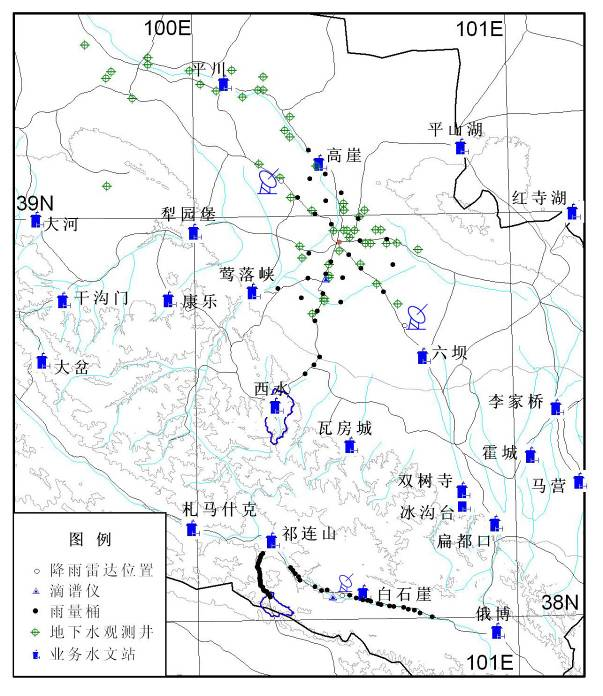
\includegraphics{hydrology_system.png}\hfill}

图X 降水径流观测系统概念图

图 X  黑河流域遥感-地面观测同步试验降雨及其他水文要素观测

表X 黑河流域遥感地面观测同步试验降水雷达观测系统
序号      观测点名称   观测点英文名称 观测点唯一标识码        仪器型号    位置信息    观测时段    观测项目    布置区域    景观类型
1
2
3

注:①

表X 黑河流域遥感地面观测同步试验滴谱仪观测系统
序号      观测点名称   仪器型号    观测点标识码  位置      观测时段    观测项目    布置区域    景观类型
1
2
注:①

表X 黑河流域遥感地面观测同步试验量雪筒观测系统
序号      观测点名称   英文名称    观测点唯一标识码        仪器型号    位置      观测时段    观测项目    布置区域    景观类型
1
2
3
4
5
6
7
8
9
10
11
12
13
14
15
16
17
18
19
20
21
22
23
24
25
26
27
28

注:①
表X 黑河流域遥感地面观测同步试验雨量计观测系统
序号      观测点     英文名称    唯一标识码   仪器型号    位置      观测时段    观测项目    布置区域    景观类型
1                               RG3-M
2                               RG3-M
3                               RG3-M
4                               RG3-M
5                               RG3-M
6                               RG3-M
7                               RG3-M
8                               RG3-M
9                               RG3-M
10                              RG3-M
11                              RG3-M
12                              RG3-M
13                              RG3-M
14                              RG3-M
15                              RG3-M
16                              RG3-M
17                              RG3-M
18                              RG3-M
19                              RG3-M
20                              RG3-M
21                              RG3-M
22                              RG3-M
23                              RG3-M
24                              RG3-M
25                              RG3-M
26                              RG3-M
27                              RG3-M
28                              RG3-M
29                              RG3-M

注:①
表X 黑河流域遥感地面观测同步试验常规水文观测系统
序号      观测站名称   观测站英文名称 观测站唯一标识码        位置      观测时段    观测项目    景观类型
1
2
3
注:①
表X 黑河流域遥感地面观测同步试验径流观测点
序号      观测点名称   观测点英文名称 仪器型号    观测地点标识码 位置      观测时段    观测项目    景观类型
1
2
3
注:①

表X 黑河流域遥感地面观测同步试验地下水观测井
序号      观测点名称   观测点英文名称 英文缩写或标识码        位置      观测时段    观测项目    所在试验区
1
2
3
注:①

表X 黑河流域遥感地面观测同步试验灌溉观测系统
序号      观测点名称   位置标识码   位置      观测时段    灌溉面积    所在试验区
1
2
3
注:①


\section{4.大气光学特性观测}
\label{water_observe_system:id5}
探空气球和大气光学特性
在试验区内通过探空及大气气溶胶、光学厚度、背景辐射亮温等观测,获取大气校正所需的水汽廓线、温度廓线、气溶胶分布、程辐射等信息
地基微波辐射计
共有两套。973 项目一套(6.925GHz(双极化),10.65GHz(双极化),18.7GHz(双极化),36.5GHz(双极化)),寒旱所一套(3GHz,5.3GHz,10.8GHz,18.7GHz,37GHz),
寒区试验布设在冰沟和阿柔乡(3-4 月份),干旱区水文试验布设在兰州大学草地站(5-7月份)。
(2) 散射计
地基散射计(13.8GHz)寒区试验布设在阿柔和扁都口(3-4 月份);干旱区水文试验布设在临泽(5-7 月份),主要观测土壤水分。
(3) 探地雷达
用于寒区水文试验中的冻融试验,布设阿柔。
(4) 光谱议
布设在各试验区,用于各种地物光谱特性的同步观测。
(5) 红外地表辐射温度
布设在各试验区,用于地表辐射温度的同步及连续观测。
(6) LAS 大孔径闪烁仪
计划在冬季布设在上游阿柔冻融观测站,夏季布设在中游兰大草地站。

图X 黑河流域遥感-地面观测同步试验大气光学特性观测系统

表X黑河流域遥感-地面观测同步试验大气光学特性观测系统
序号      观测地点    仪器型号    位置标识码   观测要素    观测时段    所在试验区   景观类型


\section{5. 积雪水文观测系统}
\label{water_observe_system:id6}

\section{6. 冻土冻融观测系统}
\label{water_observe_system:id7}

\section{7. 森林水文观测系统}
\label{water_observe_system:id8}
4.8植物生理和几何特征观测系统

4.9地面样区和样点观测系统
4.9.1上游寒区水文试验区积雪样区和采样点设置
积雪观测样地共5个,均位于冰沟小流域内。
表X黑河流域遥感-地面观测同步试验积雪观测样区位置信息
序号      样地名称    纬度      经度      海拔
1       A       38.01407        100.24295       4145
2       B       38.01255        100.23088       4138
3       C       38.01615        100.24323       4142
4       D       38.01828        100.23710       4042
5       E       38.02308        100.23202       3923
注:

4.4.2上游寒区水文试验区冻土冻融过程样区与采样点设置
土壤冻融过程观测样地6个,分别位于阿柔,扁渡口和俄堡。
表X 黑河流域遥感-地面观测同步试验冻土冻融过程样区位置信息
序号      名 称     纬 度     经 度     海 拔
1       扁渡口1    38.27900        100.91203       2673
2       扁渡口2    38.33112        100.89378       2523
3       阿柔1     38.04492        100.46656       3034
4       阿柔2     38.05667        100.47689       2994
5       俄堡1     38.00306        100.72969       3188
6       俄堡2     37.99964        100.72794       3183
注:

图X黑河流域遥感-地面观测同步试验冻土冻融过程样区

4.4.3上游寒区水文试验区花杆布置
11月11日和16日分别布设花杆51个,分别位于平坦地、阴坡、阳坡和半阴坡(包括早上向阳和下午向阳面)
表 黑河流域遥感-地面观测同步试验花杆位置信息
序号      花杆编号    纬度      经度      海拔
\begin{quote}

21      38.01403        100.24223       4147
22      38.01403        100.24260       4145
23      38.01403        100.24295       4147
24      38.01405        100.24328       4147
25      38.01403        100.24362       4147
26      38.01402        100.24397       4133
27      38.01408        100.24432       4136
28      38.01407        100.24462       4140
29      38.01403        100.24488       4142
30      38.01377        100.24363       4137
31      38.01350        100.24362       4135
32      38.01323        100.24360       4131
33      38.01297        100.24362       4129
34      38.01433        100.24362       4138
35      38.01460        100.24362       4138
36      38.01488        100.24360       4140
37      38.01513        100.24360       4140
38      38.01598        100.23835       4094
39      38.01623        100.23795       4085
40      38.01650        100.23772       4071
41      38.01682        100.23753       4059
42      38.01713        100.23737       4052
43      38.01742        100.23733       4048
44      38.01775        100.23742       4043
45      38.01803        100.23758       4039
46      38.01648        100.23635       4085
47      38.01677        100.23652       4077
48      38.01693        100.23677       4069
49      38.01712        100.23702       4060
50      38.02003        100.23565       4033
51      38.01997        100.23548       4015
52      38.02017        100.23535       4011
53      38.02042        100.23518       4005
54      38.02062        100.23503       4003
55      38.02088        100.23482       3998
56      38.02652        100.23507       4030
57      38.02637        100.23482       4023
58      38.02628        100.23482       4007
59      38.02613        100.23457       4005
60      38.02602        100.23447       4002
61      38.02583        100.23430       3981
62      38.02560        100.23427       3980
63      38.01963        100.23402       4012
64      38.01982        100.23387       4003
65      38.01998        100.23377       3991
66      38.02015        100.23368       3982
67      38.02033        100.23357       3976
68      38.02050        100.23345       3970
69      38.02068        100.23332       3960
70      38.02085        100.23318       3954
71      38.02102        100.23310       3949
\end{quote}

图 黑河流域遥感-地面观测同步试验花杆位置信息
4.4.4上游寒区水文试验区土壤水分样区
我们在阿柔埋设了快速土壤水分测量管25根。
测量管编号   纬度      精度      海拔
1       38.04523        100.46573       3030
2       38.04520        100.46608       3029
3       38.04518        100.46643       3027
4       38.04518        100.46678       3028
5       38.04503        100.46660       3028
6       38.04503        100.46623       3026
7       38.04503        100.46590       3025
8       38.04488        100.46572       3025
9       38.04490        100.46607       3027
10      38.04490        100.46643       3028
11      38.04492        100.46678       3028
12      38.04477        100.46660       3028
13      38.04477        100.46623       3027
14      38.04477        100.46587       3026
15      38.04462        100.46570       3025
16      38.04462        100.46607       3026
17      38.04463        100.46643       3027
18      38.04463        100.46680       3028
19      38.04450        100.46660       3029
20      38.04450        100.46623       3031
21      38.04448        100.46588       3028
22      38.04433        100.46568       3029
23      38.04435        100.46605       3029
24      38.04437        100.46643       3029
25      38.04437        100.46680       3031


\chapter{观测规范}
\label{observe_standard::doc}\label{observe_standard:observe-standard}\label{observe_standard:id1}

\section{方向比辐射率观测规范}
\label{observe_standard:id2}
Todo:


\section{冻土观测规范}
\label{observe_standard:id3}
Todo:


\section{土壤电导率测定规范}
\label{observe_standard:id4}
Todo:


\section{土壤含水量环刀法测量规范}
\label{observe_standard:id5}
Todo:


\section{野外光谱仪操作规范}
\label{observe_standard:id6}
Todo:


\section{野外光谱仪操作手册}
\label{observe_standard:id7}
Todo:


\section{叶面积指数(LAI)测量规范}
\label{observe_standard:lai}
Todo:


\section{叶倾角等参数测量规范}
\label{observe_standard:id8}
Todo:


\section{植被占空比测量规范}
\label{observe_standard:id9}
Todo:


\section{Delta TDR测量规范}
\label{observe_standard:delta-tdr}
Todo:


\section{Steven TDR 测量规范}
\label{observe_standard:steven-tdr}
Todo:


\section{波谱仪观测记录表}
\label{observe_standard:id10}
Todo:


\section{地表粗糙度观测规范}
\label{observe_standard:id11}
Todo:


\section{地基微波辐射计观测规范}
\label{observe_standard:id12}
Todo:


\section{多角度观测架使用规范}
\label{observe_standard:id13}
Todo:


\section{反照率表观测规范}
\label{observe_standard:id14}
Todo:


\section{红外温度及波谱测量规范}
\label{observe_standard:id15}
Todo:


\section{积分球操作规范}
\label{observe_standard:id16}
Todo:


\section{光量子计测量PAR}
\label{observe_standard:par}
Todo:


\section{结构及生理生化参数测量规范}
\label{observe_standard:id17}
Todo:


\section{超级样地测量流程}
\label{observe_standard:id18}
Todo:


\section{地基激光雷达实验手册}
\label{observe_standard:id19}
Todo:


\section{森林样地-样带观测方案与观测规范}
\label{observe_standard:id20}
Todo:


\section{手持式TDR标定比对试验规范}
\label{observe_standard:tdr}
Todo:


\section{土壤水分环刀法测量规范}
\label{observe_standard:id21}
Todo:


\section{地表反照率的测量规范}
\label{observe_standard:id22}
Todo:


\section{野外光谱仪操作规范}
\label{observe_standard:id23}
Todo:


\section{积分球操作说明}
\label{observe_standard:id24}
Todo:


\chapter{数据清单}
\label{doc_datalist:doc-datalist}\label{doc_datalist::doc}\label{doc_datalist:id1}

\section{黑河综合遥感联合试验:阿柔试验区机载微波辐射计(L\&K波段)地面同步观测数据集(2008年3月19日)}
\label{fecd46b0-3390-4580-a415-2d49ba77f9bd:fecd46b0-3390-4580-a415-2d49ba77f9bd}\label{fecd46b0-3390-4580-a415-2d49ba77f9bd:l-k-2008319}\label{fecd46b0-3390-4580-a415-2d49ba77f9bd::doc}\begin{description}
\item[{\textbf{英文标题:}}] \leavevmode
WATER: Simultaneous Airborne Microwave Radiometer (L\&K-band)-Ground Observation Dataset in A'rou Experimental Area on March 19, 2008

\end{description}


\subsection{1. 摘要}
\label{fecd46b0-3390-4580-a415-2d49ba77f9bd:id1}
2008年3月19日,在阿柔试验区开展了L\&K波段机载微波辐射计的航空飞行。 地面同步观测在微波同步样带L2、样带L4及样带L5展开。样带为南北向分布,每条样带上采样点间距约为100m。同步时自北向南行进。 在样带L2,采用POGO便携式土壤传感器获得土壤温度、土壤水分、损耗正切、土壤电导率、土壤复介电实部及虚部;针式温度计获得0-5cm平均土壤温度;并采用环刀取土经烘干获得重量含水量、体积含水量及土壤容重。 在样带L4,采用POGO便携式土壤传感器获得土壤温度、土壤水分、损耗正切、土壤电导率、土壤复介电实部及虚部;针式温度计获得0-5cm平均土壤温度;手持式热红外温度枪获得3次地表辐射温度;并采用环刀取土经烘干获得重量含水量、体积含水量及土壤容重。 在样带L5,采用ML2X土壤水分速测仪(四针)获取土壤体积含水量;针式温度计获得0-5cm平均土壤温度;并采用环刀取土经烘干获得重量含水量、体积含水量及土壤容重。此外,还在样带L4开展了手持热像仪的同步观测,在阿柔样带L6开展了GPR监测。 本数据集包括了5个文件,分别为:L\&K波段机载微波辐射数据、样带L2数据、样带L4数据、样带L5数据、探地雷达数据。其中阿柔样带L2.excel和包括Steven TDR、针式温度数据和环刀取土数据;阿柔样带L4.excel和包括Steven TDR、针式温度计数据、手持式热红外温度枪数据和环刀取土数据;阿柔样带L5.excel和包括Theta TDR(冻土)数据、针式温度计数据和环刀取土数据。 问题:请补充L\&K波段机载微波辐射数据以及探地雷达数据(请详尽描述数据信息,如数据日期、获取途径、处理过程、质量评估以及数据处理人员等)


\subsection{2. 关键词}
\label{fecd46b0-3390-4580-a415-2d49ba77f9bd:id2}\begin{description}
\item[{主题关键词:}] \leavevmode
GPR, ML2X土壤水分速测仪(四针), 针式温度计, 冻结深度, 地面同步观测, 土壤冻融, POGO便携式土壤传感器, 土壤水分, 土壤温度, 地表温度, L波段, 机载微波辐射计, 手持式热像仪, 环刀, K波段, 手持式热红外温度枪, 损耗正切, 土壤电导率, 介电常数, 土壤容重, 土壤水分速测仪, 探地雷达,

\item[{位置关键词:}] \leavevmode
上游寒区水文试验区, 阿柔试验区, 阿柔样带L2, 阿柔样带L4, 阿柔样带L5, 阿柔样带L6, 黑河流域,

\item[{时间关键词:}] \leavevmode
2008-03-19,

\end{description}

学科关键词:


\subsection{3. 本数据的引用}
\label{fecd46b0-3390-4580-a415-2d49ba77f9bd:id3}\begin{description}
\item[{中文引用:}] \leavevmode
曹永攀,顾娟,韩旭军,晋锐,李哲,王建华,王维真,吴月茹,周红敏,历华,周红敏,常存,于梅艳,赵金,雷雨田,孙继成,闫业庆.黑河综合遥感联合试验:阿柔试验区机载微波辐射计(L\&amp;K波段)地面同步观测数据集(2008年3月19日),中国西部环境与生态科学数据中心,2008.doi:10.3972/water973.xxxx.db

\item[{英文引用:}] \leavevmode
Cao Yongpan,Gu Juan,Han Xujun,Jin Rui,Li Zhe,Wang Jianhua,Wang Weizhen,Wu Yueru,Zhou Hongmin,Li Hua,Zhou Hongmin,Chang Cun,Yu Meiyan,Zhao Jin,Lei Yutian,Sun Jicheng,Yan Yeqing.WATER: Simultaneous Airborne Microwave Radiometer (L\&amp;K-band)-Ground Observation Dataset in A'rou Experimental Area on March 19, 2008,Environmental and Ecological Science Data Center for West China,2008.doi:10.3972/water973.xxxx.db

\end{description}


\subsection{4.      数据调查者}
\label{fecd46b0-3390-4580-a415-2d49ba77f9bd:id4}\begin{itemize}
\item {} 
姓名:曹永攀,顾娟,韩旭军,晋锐,李哲,王建华,王维真,吴月茹

\item {} 
单位:中国科学院寒区旱区环境与工程研究所

\item {} 
通讯地址:中国--甘肃省--兰州--兰州市东岗西路320号

\item {} 
邮编:730000

\item {} 
姓名:周红敏

\item {} 
单位:北京师范大学

\item {} 
通讯地址:中国--北京市--兰州--北京市海淀区新街口外大街19号

\item {} 
邮编:100875

\item {} 
姓名:历华,周红敏

\item {} 
单位:中国科学院遥感应用研究所

\item {} 
通讯地址:中国--北京市--兰州--北京市朝阳区大屯路中国科学院奥运村科学园区

\item {} 
邮编:100101

\item {} 
姓名:常存,于梅艳,赵金

\item {} 
单位:中国科学院新疆生态与地理研究所

\item {} 
通讯地址:中国--新疆维吾尔自治区--兰州--乌鲁木齐市北京南路40-3号

\item {} 
邮编:830011

\item {} 
姓名:雷雨田

\item {} 
单位:海德堡大学

\item {} 
通讯地址:中国--巴登-符腾堡州--兰州--69047 Heidelberg, Postfach 105760

\item {} 
邮编:105760

\item {} 
姓名:孙继成,闫业庆

\item {} 
单位:兰州大学

\item {} 
通讯地址:中国--甘肃省--兰州--兰州市天水北路210号

\item {} 
邮编:730000

\end{itemize}


\subsection{5. 数据联系人}
\label{fecd46b0-3390-4580-a415-2d49ba77f9bd:id5}\begin{itemize}
\item {} 
姓名:晋锐

\item {} 
单位:中国科学院寒区旱区环境与工程研究所

\item {} 
通讯地址:中国--甘肃省--兰州--兰州市东岗西路320号

\item {} 
邮编:730000

\item {} 
电子邮件:jinrui@lzb.ac.cn

\item {} 
电话:0931-4967298

\end{itemize}


\subsection{6. 元数据作者}
\label{fecd46b0-3390-4580-a415-2d49ba77f9bd:id6}\begin{itemize}
\item {} 
姓名:晋锐

\item {} 
单位:中国科学院寒区旱区环境与工程研究所

\item {} 
通讯地址:中国--甘肃省--兰州--兰州市东岗西路320号

\item {} 
邮编:730000

\item {} 
电子邮件:jinrui@lzb.ac.cn

\item {} 
电话:0931-4967298

\end{itemize}


\subsection{7.      元数据发布者}
\label{fecd46b0-3390-4580-a415-2d49ba77f9bd:id7}\begin{itemize}
\item {} 
姓名:吴立宗

\item {} 
单位:中国科学院寒区旱区环境与工程研究所

\item {} 
通讯地址:中国--甘肃省--兰州--兰州市东岗西路320号

\item {} 
邮编:730000

\item {} 
电子邮件:wulizong@lzb.ac.cn

\item {} 
电话:0931-4967298

\end{itemize}


\subsection{8.      数据分发者}
\label{fecd46b0-3390-4580-a415-2d49ba77f9bd:id8}\begin{itemize}
\item {} 
姓名:李红星

\item {} 
单位:中国科学院寒区旱区环境与工程研究所

\item {} 
通讯地址:中国--甘肃--兰州--兰州市东岗西路320号

\item {} 
邮编:730000

\item {} 
电子邮件:westdc@lzb.ac.cn

\item {} 
电话:0931-4967287

\item {} 
传真:0931-8279161

\end{itemize}


\subsection{9.      地理范围}
\label{fecd46b0-3390-4580-a415-2d49ba77f9bd:id9}\begin{itemize}
\item {} 
北:38.078

\item {} 
南:38.015

\item {} 
西:100.411

\item {} 
东:100.550

\end{itemize}


\subsection{10.     项目支持信息}
\label{fecd46b0-3390-4580-a415-2d49ba77f9bd:id10}\begin{description}
\item[{本试验的开展及数据的管理与发布获得了以下项目的支持:}] \leavevmode\begin{enumerate}
\item {} 
中国科学院西部行动计划(二期)项目:黑河流域遥感-地面观测同步试验与综合模拟平台建设(项目编号:KZCX2-XB2-09)

\item {} 
国家重点基础研究发展规划(973)项目:陆表生态环境要素主被动遥感协同反演理论与方法(项目编号:2007CB714400)

\end{enumerate}

\end{description}


\subsection{11. 文件清单}
\label{fecd46b0-3390-4580-a415-2d49ba77f9bd:id11}
文件路径: \code{/data/WATER/Level\_1/Arou/ARou\_Sync\_2008-03-19\_L+K}

\begin{Verbatim}[commandchars=@\[\]]
1. /照片/DSC02073.JPG
2. /K@_Band/KDATA2008-04-06-1505.dat
3. /K@_Band/KTB2008-04-06-1050.dat
4. /K@_Band/KTB2008-04-08-0937.dat
5. /K@_Band/KDATA2008-04-07-1355.dat
6. /K@_Band/KTB2008-04-06-1606.dat
7. /K@_Band/KDATA2008-04-06-2004.dat
8. /K@_Band/KTB2008-04-07-1449.dat
9. /K@_Band/K2008-04-06-1505.txt
10. /K@_Band/K2008-04-06-1606.txt
11. /K@_Band/KDATA2008-04-08-0937.dat
12. /K@_Band/KDATA2008-04-07-1534.dat
13. /K@_Band/KTB2008-04-06-2004.dat
14. /K@_Band/KTB2008-04-06-1309.dat
15. /K@_Band/KDATA2008-04-06-1209.dat
16. /K@_Band/K2008-04-07-1534.txt
17. /K@_Band/KDATA2008-04-07-1449.dat
18. /K@_Band/KDATA2008-04-07-1319.dat
19. /K@_Band/K2008-04-07-1449.txt
20. /K@_Band/K2008-04-07-1604.txt
21. /K@_Band/K2008-04-05-1157.txt
22. /K@_Band/KDATA2008-04-06-1606.dat
23. /K@_Band/KTB2008-04-07-1319.dat
24. /K@_Band/KDATA2008-04-05-1157.dat
25. /K@_Band/KTB2008-04-07-1534.dat
26. /K@_Band/KDATA2008-04-07-1604.dat
27. /K@_Band/K2008-04-06-1209.txt
28. /照片/
29. /照片/DSC02075.JPG
30. /照片/DSC02076.JPG
31. /照片/DSC02079.JPG
32. /照片/DSC02074.JPG
33. /照片/DSC02082.JPG
34. /照片/DSC02080.JPG
35. /照片/DSC02077.JPG
36. /照片/DSC02072.JPG
37. /照片/DSC02078.JPG
38. /照片/DSC02081.JPG
39. /Ka@_Band/
40. /Ka@_Band/KaDATA2008-04-05-1201.dat
41. /Ka@_Band/KaTB2008-04-05-1804.dat
42. /Ka@_Band/KaDATA2008-04-05-1804.dat
43. /Ka@_Band/Ka2008-04-05-1201.txt
44. /Ka@_Band/Ka2008-04-05-1804.txt
45. /Ka@_Band/KaTB2008-04-05-1201.dat
46. /S@_Band/
47. /S@_Band/S2008-04-06-2006.txt
48. /S@_Band/S2008-04-07-1317.txt
49. /S@_Band/SDATA2008-04-06-1208.dat
50. /S@_Band/S2008-04-06-2015.txt
51. /S@_Band/S2008-04-06-1310.txt
52. /S@_Band/STB2008-04-07-1456.dat
53. /S@_Band/STB2008-04-06-1310.dat
54. /S@_Band/S2008-04-07-1456.txt
55. /S@_Band/STB2008-04-06-1208.dat
56. /S@_Band/S2008-04-06-1052.txt
57. /S@_Band/SDATA2008-04-07-1535.dat
58. /S@_Band/STB2008-04-07-1605.dat
59. /S@_Band/STB2008-04-08-1006.dat
60. /S@_Band/STB2008-04-07-1535.dat
61. /S@_Band/S2008-04-07-1535.txt
62. /S@_Band/SDATA2008-04-07-1317.dat
63. /S@_Band/S2008-04-06-1506.txt
64. /S@_Band/STB2008-04-07-1317.dat
65. /S@_Band/STB2008-04-06-2015.dat
66. /S@_Band/STB2008-04-06-2006.dat
67. /S@_Band/SDATA2008-04-06-1407.dat
68. /S@_Band/S2008-04-06-1605.txt
69. /S@_Band/SDATA2008-04-07-1605.dat
70. /S@_Band/S2008-04-06-1208.txt
71. /S@_Band/STB2008-04-07-1355.dat
72. /S@_Band/SDATA2008-04-06-2006.dat
73. /S@_Band/STB2008-04-06-1605.dat
74. /S@_Band/SDATA2008-04-06-1605.dat
75. /S@_Band/SDATA2008-04-08-1006.dat
76. /S@_Band/STB2008-04-06-1407.dat
77. /S@_Band/SDATA2008-04-07-1355.dat
78. /S@_Band/SDATA2008-04-06-1506.dat
79. /S@_Band/S2008-04-07-1355.txt
80. /S@_Band/SDATA2008-04-07-1456.dat
81. /S@_Band/SDATA2008-04-06-2015.dat
82. /S@_Band/S2008-04-08-1006.txt
83. /S@_Band/S2008-04-06-1407.txt
84. /S@_Band/SDATA2008-04-06-1310.dat
85. /S@_Band/S2008-04-07-1605.txt
86. /S@_Band/STB2008-04-06-1506.dat
87. /S@_Band/SDATA2008-04-06-1052.dat
88. /S@_Band/STB2008-04-06-1052.dat
89. /定标系数/
90. /定标系数/X波段微波辐射计定标系数.txt
91. /定标系数/S波段微波辐射计定标系数.txt
92. /定标系数/C波段微波辐射计定标系数.txt
93. /定标系数/K波段微波辐射计定标系数.txt
94. /定标系数/Ka波段微波辐射计定标系数.txt
95. /C@_Band/
96. /C@_Band/CTB2008-04-08-0959.dat
97. /C@_Band/CTB2008-04-07-1530.dat
98. /C@_Band/CDATA2008-04-08-0959.dat
99. /C@_Band/C2008-04-07-1530.txt
100. /C@_Band/CDATA2008-04-07-1530.dat
101. /C@_Band/C2008-04-08-0959.txt
102. /阿柔微波辐射计观测场土壤温湿度自动观测(20080405-20080408).xls
103. /观测记录.doc
104. /阿柔微波辐射计观测场地温人工观测(20080405-20080408).xls
105. /K@_Band/
106. /K@_Band/K2008-04-06-1309.txt
107. /K@_Band/K2008-04-06-2004.txt
108. /K@_Band/KDATA2008-04-06-1407.dat
109. /K@_Band/K2008-04-07-1355.txt
110. /K@_Band/KTB2008-04-06-1407.dat
111. /K@_Band/KTB2008-04-06-1209.dat
112. /K@_Band/K2008-04-06-1407.txt
113. /K@_Band/KTB2008-04-06-1505.dat
114. /K@_Band/KTB2008-04-07-1604.dat
115. /K@_Band/KTB2008-04-05-1157.dat
116. /K@_Band/KDATA2008-04-06-1309.dat
117. /K@_Band/K2008-04-07-1319.txt
118. /K@_Band/K2008-04-06-1050.txt
119. /K@_Band/KTB2008-04-07-1355.dat
120. /K@_Band/KDATA2008-04-06-1050.dat
121. /K@_Band/K2008-04-08-0937.txt
122. /阿柔样带5.xls
123. /阿柔样带4.xls
124. /请补充L@&K波段机载微波辐射数据和探地雷达数据/
125. /阿柔样带2.xls
\end{Verbatim}


\chapter{如何获取数据}
\label{data_acquire:id1}\label{data_acquire::doc}\label{data_acquire:data-acquire}

\section{1. 通过西部数据中心获取数据}
\label{data_acquire:id2}
“西部数据中心”是国家自然科学基金委员会“中国西部环境与生态科学研究计划”以建设集成化、体系化、规范化科学数据共享平台为目标而设立的重点研究项目,承担“西部计划”项目数据产出的收集、管理、集成,并面向西部环境与生态科学的各个领域提供科学数据服务。

其数据共享平台定位于数据集的管理发布并面向数据用户提供数据信息和数据服务。根据共享平台的实现,选择了国际元数据标准ISO 19115作为“黑河综合联合遥感实验”的元数据标准,依靠灵活的数据快速导航系统,实现了空间数据的不同导航模式,包括分类、关键词、数据集序列、时间和空间导航方式,实现了空间数据的快速搜索、浏览,可以让用户快速的找到所需的数据。


\subsection{1.1 用户注册}
\label{data_acquire:id3}

\subsection{1.2 检索数据}
\label{data_acquire:id4}

\subsubsection{A. 基于类别的数据导航}
\label{data_acquire:a}
{\hfill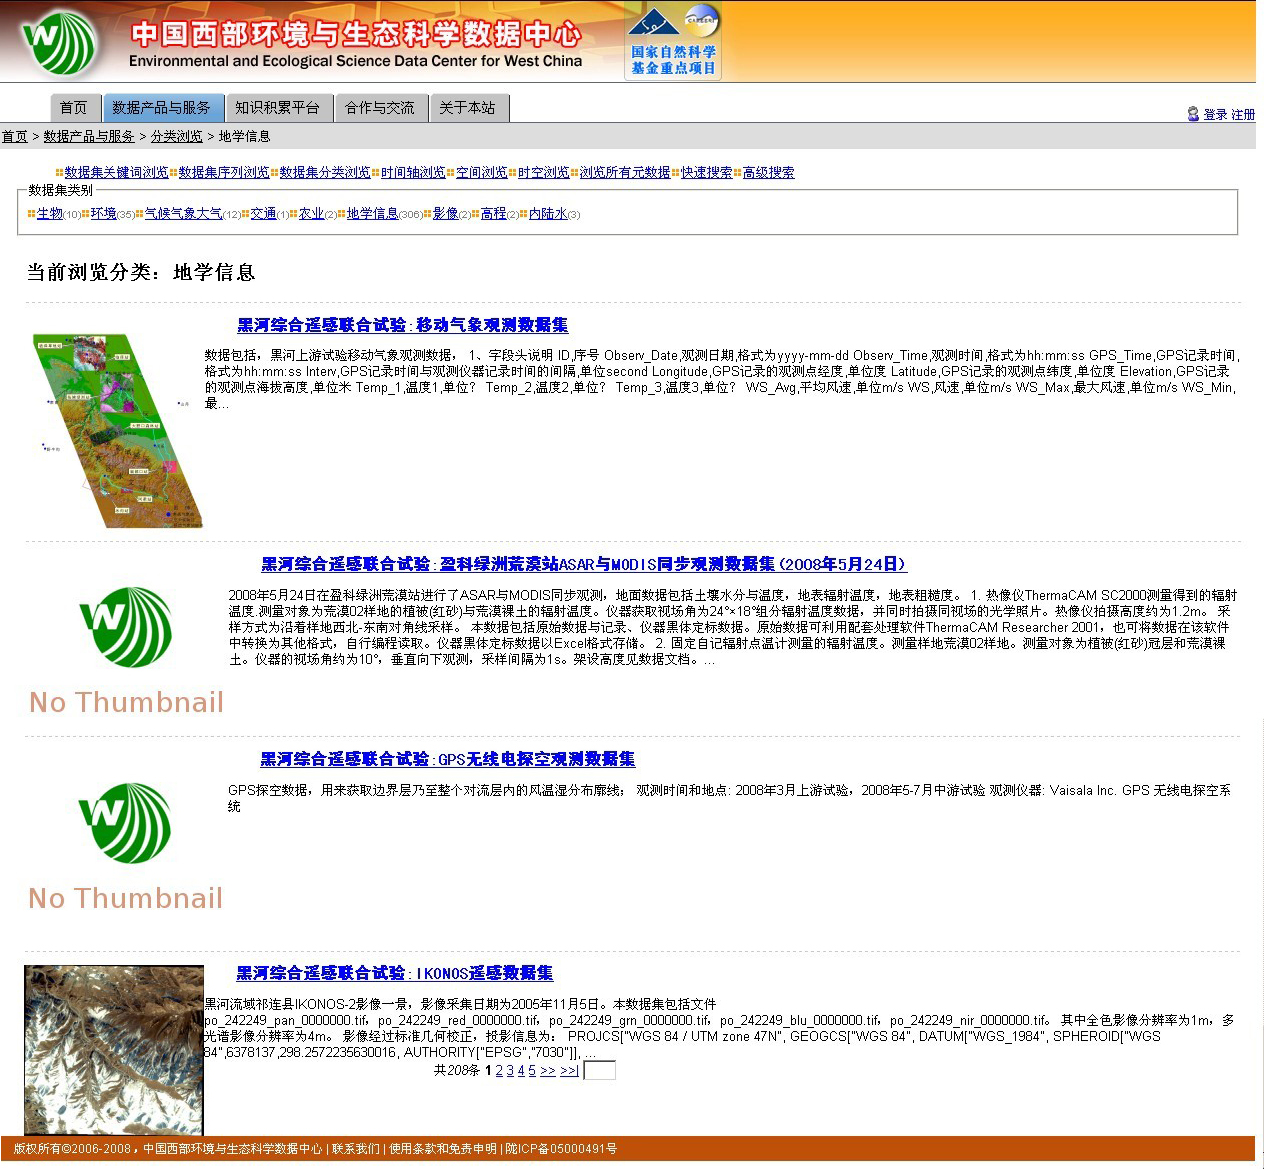
\includegraphics{westdc_nav_class.jpg}\hfill}


\subsubsection{B. 基于关键词的数据导航}
\label{data_acquire:b}
{\hfill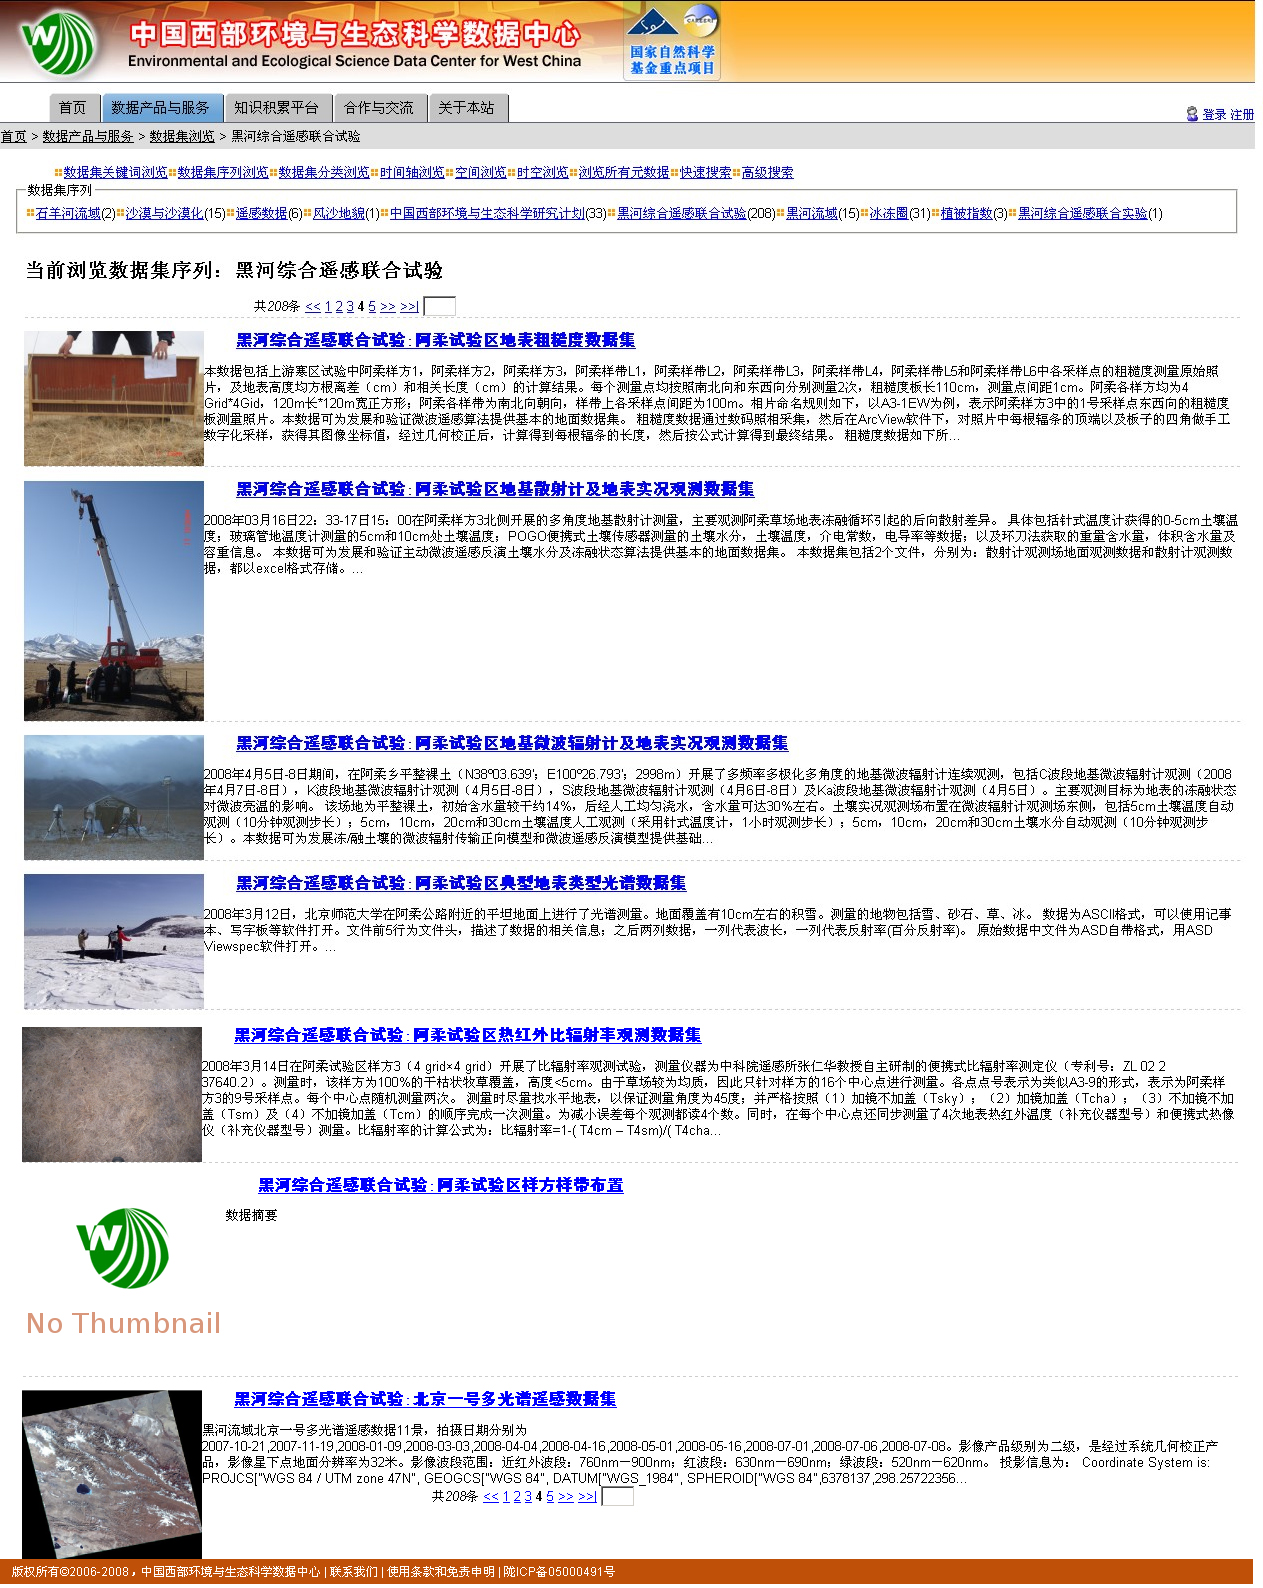
\includegraphics{westdc_nav_keyword.jpg}\hfill}


\subsubsection{C. 基于时间的数据导航}
\label{data_acquire:c}
{\hfill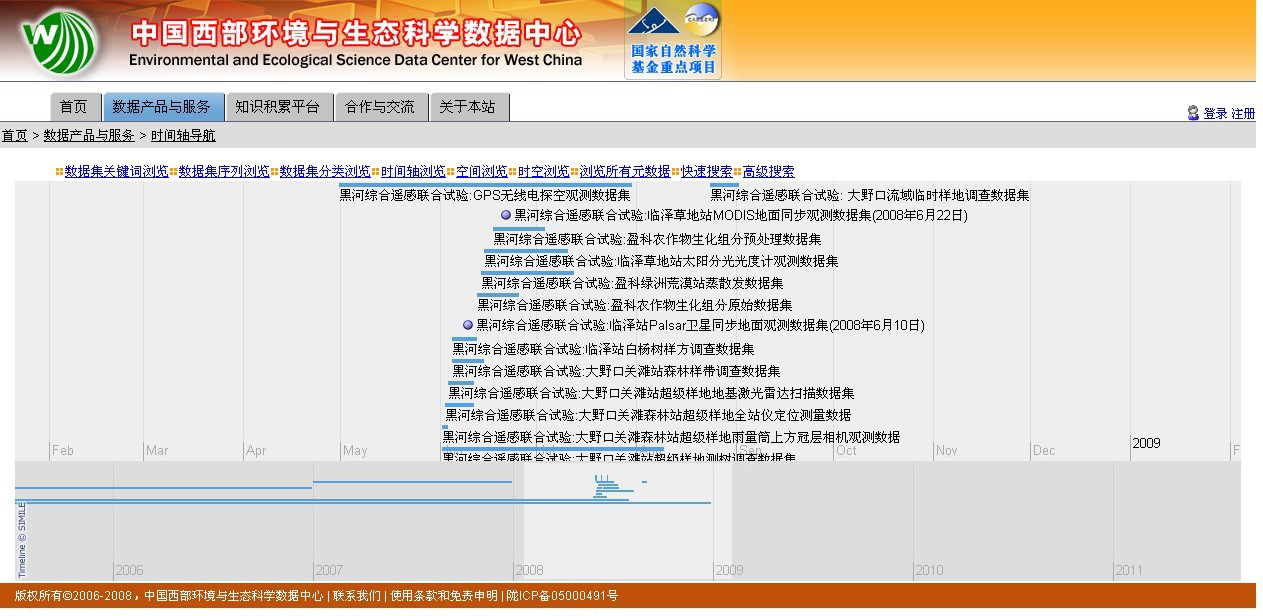
\includegraphics{westdc_nav_time.jpg}\hfill}


\subsubsection{D. 基于空间的数据导航}
\label{data_acquire:d}
{\hfill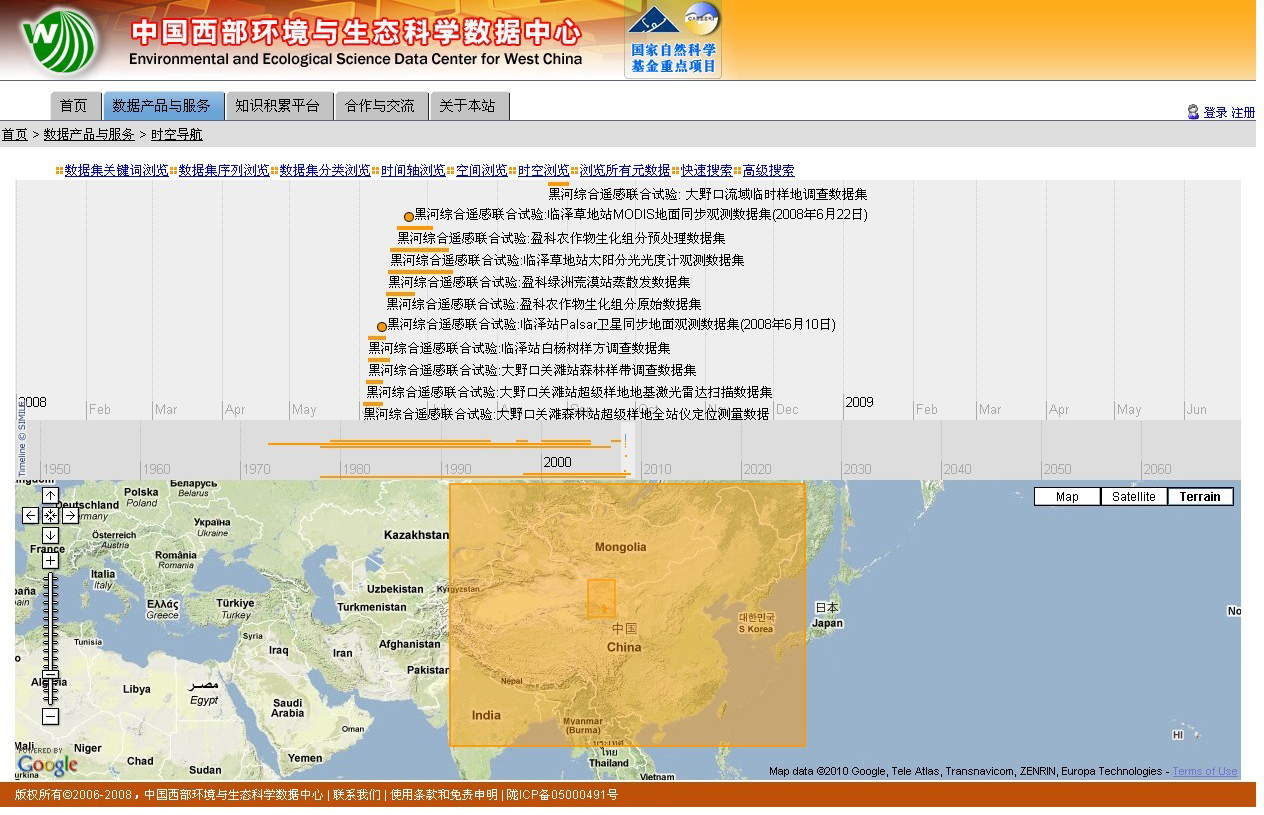
\includegraphics{westdc_nav_space.jpg}\hfill}


\subsection{1.3 填写数据申请表}
\label{data_acquire:id5}

\subsection{1.4 下载数据}
\label{data_acquire:id6}

\section{2.通过北京师范大学下载}
\label{data_acquire:id7}

\chapter{试验日志}
\label{water_blog:water-blog}\label{water_blog::doc}\label{water_blog:id1}
Todo


\chapter{组织单位与参加人员}
\label{water_partner::doc}\label{water_partner:doc-arou}\label{water_partner:id1}

\section{组织单位}
\label{water_partner:id2}

\subsection{中国科学院寒区旱区环境与工程研究所}
\label{water_partner:id3}\begin{description}
\item[{\textbf{通讯地址:}}] \leavevmode
兰州市东岗西路320号,730000

\item[{\textbf{参加者:}}] \leavevmode
白艳芬
白云洁
曹永攀
钞振华
车涛
楚荣忠
崔文瑞
戴礼云
丁松爽
杜自强
盖春梅
盖迎春
高洪春
高松
高艳红
谷良雷
顾娟
韩旭军
郝晓华
何慧根
侯旭宏
胡晓利
胡泽勇
黄春林
贾伟
蒋熹
晋锐
李弘毅
李红星
李建成
李茂善
李新
李哲
梁继
刘超
马明国
马伟强
马晓伟
年雁云
潘小多
钱金波
秦春
冉有华
任燕霞
舒乐乐
宋怡
苏培玺
孙方林
谭俊磊
汤瀚
汪洋
王建
王建华
王介民
王亮绪
王树果
王维真
王旭峰
王应贵
王之夏
王志宏
王致君
吴立宗
吴月茹
辛秉洁
徐瑱
严巧娣
张岭梅
张彤
赵果
钟兰鸿
周秀云
朱仕杰

\end{description}


\subsection{中国科学院遥感应用研究所}
\label{water_partner:id4}\begin{description}
\item[{\textbf{通讯地址:}}] \leavevmode
北京市朝阳区大屯路中国科学院奥运村科学园区,100101

\item[{\textbf{参加者:}}] \leavevmode
鲍云飞
曹春香
陈雪
董晶晶
杜永明
方莉
付安民
高帅
龚建华
光洁
何祺胜
李丽
李利伟
李莎
李小文
李祖传
历华
刘晨州
刘强
刘思含
刘雅妮
柳钦火
路鹏
吕永红
倪文俭
牛铮
彭菁菁
苏高利
孙国清
覃驭楚
王殿中
王合顺
王莉雯
王新云
王颖
闻建光
邬明权
吴朝阳
夏传福
肖青
辛晓洲
杨习荣
殷小军
袁金国
占玉林
张颢
张阳
张志玉
支毅乔
周春艳
周红敏
周梦维

\end{description}


\subsection{北京师范大学}
\label{water_partner:id5}\begin{description}
\item[{\textbf{通讯地址:}}] \leavevmode
北京市海淀区新街口外大街19号,100875

\item[{\textbf{参加者:}}] \leavevmode
柏延臣
柴源
常胜
常燕
陈玲
董建
房倩
付卓
郭新平
何涛
瞿瑛
康国婷
李波
李静
李小文
李欣欣
厉香蕴
梁星涛
林皓波
刘绍民
刘素红
刘誉
刘志刚
潘金梅
彭丹青
钱永刚
曲伟
屈永华
任华忠
任杰
任智星
双喜
宋旦霞
宋金玲
孙青松
孙小青
孙志超
王颢星
王锦地
王天星
肖月庭
肖志强
徐自为
阎广建
姚冬萍
余莹洁
张立新
张吴明
张勇攀
张志玉
赵少杰
赵天杰
郑越
周红敏
周纪
周济
朱凌
邹杰

\end{description}


\subsection{中国林业科学研究院}
\label{water_partner:id6}\begin{description}
\item[{\textbf{通讯地址:}}] \leavevmode
北京市海淀区颐和园后中国林业科学研究院,100091

\item[{\textbf{参加者:}}] \leavevmode
白黎娜
曹斌
陈尔学
高志海
过志峰
李增元
梁大双
凌飞龙
刘清旺
谭炳香
田昕
王琫瑜
王强
杨永恬
赵丽琼

\end{description}


\section{参与单位}
\label{water_partner:id7}

\subsection{成都电子科技大学}
\label{water_partner:id8}\begin{description}
\item[{\textbf{通讯地址:}}] \leavevmode
成都市建设北路二段四号,610054

\item[{\textbf{参加者:}}] \leavevmode
陈彦
黄波
贾明权
姜浩
李世华
李亚美
刘军
刘增灿
吕阳
罗震
秦伟
田雨
童玲
肖乾斌
徐春亮
许文波
杨佑禄
赵紫正

\end{description}


\subsection{中国科学院上海技术物理研究所}
\label{water_partner:id9}\begin{description}
\item[{\textbf{通讯地址:}}] \leavevmode
上海市玉田路500号,200083

\item[{\textbf{参加者:}}] \leavevmode
卜弘毅
杜奇
李正文
刘强
毛闵军
潘明忠
舒嵘
王志和
肖功海
谢锋
徐卫明
杨一德
姚波

\end{description}


\subsection{中国科学院地理科学与资源研究所}
\label{water_partner:id10}\begin{description}
\item[{\textbf{通讯地址:}}] \leavevmode
北京市朝阳区大屯路甲11号,100101

\item[{\textbf{参加者:}}] \leavevmode
陈少辉
刘照言
孙进霞
唐伯惠
唐荣林
田静
张仁华
赵伟

\end{description}


\subsection{甘肃省祁连山水源涵养林研究院}
\label{water_partner:id11}\begin{description}
\item[{\textbf{通讯地址:}}] \leavevmode
甘肃省张掖市东街,734000

\item[{\textbf{参加者:}}] \leavevmode
车宗玺
金铭
敬文茂
雷军
刘贤德
罗龙发
牛赟
王荣新
王顺利
张学龙
赵明

\end{description}


\subsection{中国科学院研究生院}
\label{water_partner:id12}\begin{description}
\item[{\textbf{通讯地址:}}] \leavevmode
北京市石景山区玉泉路甲11号,100101

\item[{\textbf{参加者:}}] \leavevmode
冯磊
李新辉
梁文广
余凡
赵英时
朱小华

\end{description}


\subsection{中国科学院新疆生态与地理研究所}
\label{water_partner:id13}\begin{description}
\item[{\textbf{通讯地址:}}] \leavevmode
乌鲁木齐市北京南路40-3号,830011

\item[{\textbf{参加者:}}] \leavevmode
常存
窦燕
解婷婷
马忠国
于梅艳
赵金

\end{description}


\subsection{北京大学}
\label{water_partner:id14}\begin{description}
\item[{\textbf{通讯地址:}}] \leavevmode
北京市海淀区颐和园路5号,100871

\item[{\textbf{参加者:}}] \leavevmode
范闻捷
刘晓臣
沈心一
陶欣
闫彬彦
姚延娟

\end{description}


\subsection{兰州大学}
\label{water_partner:id15}\begin{description}
\item[{\textbf{通讯地址:}}] \leavevmode
兰州市天水北路210号,730000

\item[{\textbf{参加者:}}] \leavevmode
马宏伟
孙继成
闫业庆
袁小龙

\end{description}


\subsection{南京大学}
\label{water_partner:id16}\begin{description}
\item[{\textbf{通讯地址:}}] \leavevmode
南京市汉口路22号,210093

\item[{\textbf{参加者:}}] \leavevmode
冯学智
姜腾龙
肖鹏峰
赵书河

\end{description}


\subsection{中国科学院东北地理与农业生态研究所}
\label{water_partner:id17}\begin{description}
\item[{\textbf{通讯地址:}}] \leavevmode
长春市高新区蔚山路3195号,800062

\item[{\textbf{参加者:}}] \leavevmode
金吉南
赵凯

\end{description}


\subsection{中国气象局兰州气象干旱研究所}
\label{water_partner:id18}\begin{description}
\item[{\textbf{通讯地址:}}] \leavevmode
甘肃省兰州市东岗东路2070号,730020

\item[{\textbf{参加者:}}] \leavevmode
韩辉
王静
王小平

\end{description}


\subsection{中国科学院对地观测与数字地球科学中心}
\label{water_partner:id19}\begin{description}
\item[{\textbf{通讯地址:}}] \leavevmode
北京市海淀区中关村北一条9号科电大厦,100190

\item[{\textbf{参加者:}}] \leavevmode
程占慧
刘良云

\end{description}


\subsection{中国科学院空间科学与应用研究中心}
\label{water_partner:id20}\begin{description}
\item[{\textbf{通讯地址:}}] \leavevmode
北京市海淀区中关村南二条一号,100190''

\item[{\textbf{参加者:}}] \leavevmode
孙波

\end{description}


\subsection{海德堡大学}
\label{water_partner:id21}\begin{description}
\item[{\textbf{通讯地址:}}] \leavevmode
69047 Heidelberg, Postfach,German 105760

\item[{\textbf{参加者:}}] \leavevmode
雷雨田

\end{description}


\subsection{中国气象局乌鲁木齐沙漠气象研究所}
\label{water_partner:id22}\begin{description}
\item[{\textbf{通讯地址:}}] \leavevmode
中国新疆乌鲁木齐市建国路46号,830002

\item[{\textbf{参加者:}}] \leavevmode
刘燕
张璞

\end{description}


\subsection{中国农业科学院}
\label{water_partner:id23}\begin{description}
\item[{\textbf{通讯地址:}}] \leavevmode
北京市海淀区中关村南大街12号中国农业科学院,100081

\item[{\textbf{参加者:}}] \leavevmode
杨贵军

\end{description}


\subsection{国家农业信息化工程技术研究中心}
\label{water_partner:id24}\begin{description}
\item[{\textbf{通讯地址:}}] \leavevmode
北京市海淀区曙光花园中路11号北京农科大厦A519,100097

\item[{\textbf{参加者:}}] \leavevmode
王大成
王纪华

\end{description}


\subsection{华南农业大学}
\label{water_partner:id25}\begin{description}
\item[{\textbf{通讯地址:}}] \leavevmode
广州市天河区五山,510640

\item[{\textbf{参加者:}}] \leavevmode
李笑宇

\end{description}


\subsection{武汉大学}
\label{water_partner:id26}\begin{description}
\item[{\textbf{通讯地址:}}] \leavevmode
武汉市武昌区东湖路8号,430072

\item[{\textbf{参加者:}}] \leavevmode
龚浩
朱满

\end{description}


\subsection{首都师范大学}
\label{water_partner:id27}\begin{description}
\item[{\textbf{通讯地址:}}] \leavevmode
北京市西三环北路105号,100048

\item[{\textbf{参加者:}}] \leavevmode
钟若飞

\end{description}


\subsection{四川师范大学}
\label{water_partner:id28}\begin{description}
\item[{\textbf{通讯地址:}}] \leavevmode
成都市锦江区静安路5号,610068

\item[{\textbf{参加者:}}] \leavevmode
杨存建

\end{description}


\subsection{兰州交通大学}
\label{water_partner:id29}\begin{description}
\item[{\textbf{通讯地址:}}] \leavevmode
兰州市安宁区安宁西路88号,730070

\item[{\textbf{参加者:}}] \leavevmode
杨天付

\end{description}


\section{支撑单位}
\label{water_partner:id30}

\subsection{中国飞行试验研究院中飞通用航空公司}
\label{water_partner:id31}\begin{description}
\item[{\textbf{通讯地址:}}] \leavevmode
西安市阎良区凌云路5号,710089

\item[{\textbf{参加者:}}] \leavevmode
陈刚
黎金宝
梁机械师
刘机长
吕良
孟机械师
潘机械师
肖机长

\end{description}


\subsection{广西桂能信息工程有限公司}
\label{water_partner:id32}\begin{description}
\item[{\textbf{通讯地址:}}] \leavevmode
广西南宁市建政路10号,530003

\item[{\textbf{参加者:}}] \leavevmode
曾林辉
钟开田
钟振云
朱能创

\end{description}


\subsection{北京天诺基业科技有限公司}
\label{water_partner:id33}\begin{description}
\item[{\textbf{通讯地址:}}] \leavevmode
北京市海淀区车公庄西路乙19号华通大厦B座北塔1222,100097

\item[{\textbf{参加者:}}] \leavevmode
胡文清
张强
赵小军

\end{description}


\section{其他人员}
\label{water_partner:id34}\begin{description}
\item[{\textbf{参加者:}}] \leavevmode
刘正虎
张楠
赵国飞

\end{description}


\chapter{黑河综合遥感联合试验:阿柔试验区机载微波辐射计(L\&K波段)地面同步观测数据集(2008年3月19日)}
\label{fecd46b0-3390-4580-a415-2d49ba77f9bd:fecd46b0-3390-4580-a415-2d49ba77f9bd}\label{fecd46b0-3390-4580-a415-2d49ba77f9bd:l-k-2008319}\label{fecd46b0-3390-4580-a415-2d49ba77f9bd::doc}\begin{description}
\item[{\textbf{英文标题:}}] \leavevmode
WATER: Simultaneous Airborne Microwave Radiometer (L\&K-band)-Ground Observation Dataset in A'rou Experimental Area on March 19, 2008

\end{description}


\section{1. 摘要}
\label{fecd46b0-3390-4580-a415-2d49ba77f9bd:id1}
2008年3月19日,在阿柔试验区开展了L\&K波段机载微波辐射计的航空飞行。 地面同步观测在微波同步样带L2、样带L4及样带L5展开。样带为南北向分布,每条样带上采样点间距约为100m。同步时自北向南行进。 在样带L2,采用POGO便携式土壤传感器获得土壤温度、土壤水分、损耗正切、土壤电导率、土壤复介电实部及虚部;针式温度计获得0-5cm平均土壤温度;并采用环刀取土经烘干获得重量含水量、体积含水量及土壤容重。 在样带L4,采用POGO便携式土壤传感器获得土壤温度、土壤水分、损耗正切、土壤电导率、土壤复介电实部及虚部;针式温度计获得0-5cm平均土壤温度;手持式热红外温度枪获得3次地表辐射温度;并采用环刀取土经烘干获得重量含水量、体积含水量及土壤容重。 在样带L5,采用ML2X土壤水分速测仪(四针)获取土壤体积含水量;针式温度计获得0-5cm平均土壤温度;并采用环刀取土经烘干获得重量含水量、体积含水量及土壤容重。此外,还在样带L4开展了手持热像仪的同步观测,在阿柔样带L6开展了GPR监测。 本数据集包括了5个文件,分别为:L\&K波段机载微波辐射数据、样带L2数据、样带L4数据、样带L5数据、探地雷达数据。其中阿柔样带L2.excel和包括Steven TDR、针式温度数据和环刀取土数据;阿柔样带L4.excel和包括Steven TDR、针式温度计数据、手持式热红外温度枪数据和环刀取土数据;阿柔样带L5.excel和包括Theta TDR(冻土)数据、针式温度计数据和环刀取土数据。 问题:请补充L\&K波段机载微波辐射数据以及探地雷达数据(请详尽描述数据信息,如数据日期、获取途径、处理过程、质量评估以及数据处理人员等)


\section{2. 关键词}
\label{fecd46b0-3390-4580-a415-2d49ba77f9bd:id2}\begin{description}
\item[{主题关键词:}] \leavevmode
GPR, ML2X土壤水分速测仪(四针), 针式温度计, 冻结深度, 地面同步观测, 土壤冻融, POGO便携式土壤传感器, 土壤水分, 土壤温度, 地表温度, L波段, 机载微波辐射计, 手持式热像仪, 环刀, K波段, 手持式热红外温度枪, 损耗正切, 土壤电导率, 介电常数, 土壤容重, 土壤水分速测仪, 探地雷达,

\item[{位置关键词:}] \leavevmode
上游寒区水文试验区, 阿柔试验区, 阿柔样带L2, 阿柔样带L4, 阿柔样带L5, 阿柔样带L6, 黑河流域,

\item[{时间关键词:}] \leavevmode
2008-03-19,

\end{description}

学科关键词:


\section{3. 本数据的引用}
\label{fecd46b0-3390-4580-a415-2d49ba77f9bd:id3}\begin{description}
\item[{中文引用:}] \leavevmode
曹永攀,顾娟,韩旭军,晋锐,李哲,王建华,王维真,吴月茹,周红敏,历华,周红敏,常存,于梅艳,赵金,雷雨田,孙继成,闫业庆.黑河综合遥感联合试验:阿柔试验区机载微波辐射计(L\&amp;K波段)地面同步观测数据集(2008年3月19日),中国西部环境与生态科学数据中心,2008.doi:10.3972/water973.xxxx.db

\item[{英文引用:}] \leavevmode
Cao Yongpan,Gu Juan,Han Xujun,Jin Rui,Li Zhe,Wang Jianhua,Wang Weizhen,Wu Yueru,Zhou Hongmin,Li Hua,Zhou Hongmin,Chang Cun,Yu Meiyan,Zhao Jin,Lei Yutian,Sun Jicheng,Yan Yeqing.WATER: Simultaneous Airborne Microwave Radiometer (L\&amp;K-band)-Ground Observation Dataset in A'rou Experimental Area on March 19, 2008,Environmental and Ecological Science Data Center for West China,2008.doi:10.3972/water973.xxxx.db

\end{description}


\section{4.      数据调查者}
\label{fecd46b0-3390-4580-a415-2d49ba77f9bd:id4}\begin{itemize}
\item {} 
姓名:曹永攀,顾娟,韩旭军,晋锐,李哲,王建华,王维真,吴月茹

\item {} 
单位:中国科学院寒区旱区环境与工程研究所

\item {} 
通讯地址:中国--甘肃省--兰州--兰州市东岗西路320号

\item {} 
邮编:730000

\item {} 
姓名:周红敏

\item {} 
单位:北京师范大学

\item {} 
通讯地址:中国--北京市--兰州--北京市海淀区新街口外大街19号

\item {} 
邮编:100875

\item {} 
姓名:历华,周红敏

\item {} 
单位:中国科学院遥感应用研究所

\item {} 
通讯地址:中国--北京市--兰州--北京市朝阳区大屯路中国科学院奥运村科学园区

\item {} 
邮编:100101

\item {} 
姓名:常存,于梅艳,赵金

\item {} 
单位:中国科学院新疆生态与地理研究所

\item {} 
通讯地址:中国--新疆维吾尔自治区--兰州--乌鲁木齐市北京南路40-3号

\item {} 
邮编:830011

\item {} 
姓名:雷雨田

\item {} 
单位:海德堡大学

\item {} 
通讯地址:中国--巴登-符腾堡州--兰州--69047 Heidelberg, Postfach 105760

\item {} 
邮编:105760

\item {} 
姓名:孙继成,闫业庆

\item {} 
单位:兰州大学

\item {} 
通讯地址:中国--甘肃省--兰州--兰州市天水北路210号

\item {} 
邮编:730000

\end{itemize}


\section{5. 数据联系人}
\label{fecd46b0-3390-4580-a415-2d49ba77f9bd:id5}\begin{itemize}
\item {} 
姓名:晋锐

\item {} 
单位:中国科学院寒区旱区环境与工程研究所

\item {} 
通讯地址:中国--甘肃省--兰州--兰州市东岗西路320号

\item {} 
邮编:730000

\item {} 
电子邮件:jinrui@lzb.ac.cn

\item {} 
电话:0931-4967298

\end{itemize}


\section{6. 元数据作者}
\label{fecd46b0-3390-4580-a415-2d49ba77f9bd:id6}\begin{itemize}
\item {} 
姓名:晋锐

\item {} 
单位:中国科学院寒区旱区环境与工程研究所

\item {} 
通讯地址:中国--甘肃省--兰州--兰州市东岗西路320号

\item {} 
邮编:730000

\item {} 
电子邮件:jinrui@lzb.ac.cn

\item {} 
电话:0931-4967298

\end{itemize}


\section{7.      元数据发布者}
\label{fecd46b0-3390-4580-a415-2d49ba77f9bd:id7}\begin{itemize}
\item {} 
姓名:吴立宗

\item {} 
单位:中国科学院寒区旱区环境与工程研究所

\item {} 
通讯地址:中国--甘肃省--兰州--兰州市东岗西路320号

\item {} 
邮编:730000

\item {} 
电子邮件:wulizong@lzb.ac.cn

\item {} 
电话:0931-4967298

\end{itemize}


\section{8.      数据分发者}
\label{fecd46b0-3390-4580-a415-2d49ba77f9bd:id8}\begin{itemize}
\item {} 
姓名:李红星

\item {} 
单位:中国科学院寒区旱区环境与工程研究所

\item {} 
通讯地址:中国--甘肃--兰州--兰州市东岗西路320号

\item {} 
邮编:730000

\item {} 
电子邮件:westdc@lzb.ac.cn

\item {} 
电话:0931-4967287

\item {} 
传真:0931-8279161

\end{itemize}


\section{9.      地理范围}
\label{fecd46b0-3390-4580-a415-2d49ba77f9bd:id9}\begin{itemize}
\item {} 
北:38.078

\item {} 
南:38.015

\item {} 
西:100.411

\item {} 
东:100.550

\end{itemize}


\section{10.     项目支持信息}
\label{fecd46b0-3390-4580-a415-2d49ba77f9bd:id10}\begin{description}
\item[{本试验的开展及数据的管理与发布获得了以下项目的支持:}] \leavevmode\begin{enumerate}
\item {} 
中国科学院西部行动计划(二期)项目:黑河流域遥感-地面观测同步试验与综合模拟平台建设(项目编号:KZCX2-XB2-09)

\item {} 
国家重点基础研究发展规划(973)项目:陆表生态环境要素主被动遥感协同反演理论与方法(项目编号:2007CB714400)

\end{enumerate}

\end{description}


\section{11. 文件清单}
\label{fecd46b0-3390-4580-a415-2d49ba77f9bd:id11}
文件路径: \code{/data/WATER/Level\_1/Arou/ARou\_Sync\_2008-03-19\_L+K}

\begin{Verbatim}[commandchars=@\[\]]
1. /照片/DSC02073.JPG
2. /K@_Band/KDATA2008-04-06-1505.dat
3. /K@_Band/KTB2008-04-06-1050.dat
4. /K@_Band/KTB2008-04-08-0937.dat
5. /K@_Band/KDATA2008-04-07-1355.dat
6. /K@_Band/KTB2008-04-06-1606.dat
7. /K@_Band/KDATA2008-04-06-2004.dat
8. /K@_Band/KTB2008-04-07-1449.dat
9. /K@_Band/K2008-04-06-1505.txt
10. /K@_Band/K2008-04-06-1606.txt
11. /K@_Band/KDATA2008-04-08-0937.dat
12. /K@_Band/KDATA2008-04-07-1534.dat
13. /K@_Band/KTB2008-04-06-2004.dat
14. /K@_Band/KTB2008-04-06-1309.dat
15. /K@_Band/KDATA2008-04-06-1209.dat
16. /K@_Band/K2008-04-07-1534.txt
17. /K@_Band/KDATA2008-04-07-1449.dat
18. /K@_Band/KDATA2008-04-07-1319.dat
19. /K@_Band/K2008-04-07-1449.txt
20. /K@_Band/K2008-04-07-1604.txt
21. /K@_Band/K2008-04-05-1157.txt
22. /K@_Band/KDATA2008-04-06-1606.dat
23. /K@_Band/KTB2008-04-07-1319.dat
24. /K@_Band/KDATA2008-04-05-1157.dat
25. /K@_Band/KTB2008-04-07-1534.dat
26. /K@_Band/KDATA2008-04-07-1604.dat
27. /K@_Band/K2008-04-06-1209.txt
28. /照片/
29. /照片/DSC02075.JPG
30. /照片/DSC02076.JPG
31. /照片/DSC02079.JPG
32. /照片/DSC02074.JPG
33. /照片/DSC02082.JPG
34. /照片/DSC02080.JPG
35. /照片/DSC02077.JPG
36. /照片/DSC02072.JPG
37. /照片/DSC02078.JPG
38. /照片/DSC02081.JPG
39. /Ka@_Band/
40. /Ka@_Band/KaDATA2008-04-05-1201.dat
41. /Ka@_Band/KaTB2008-04-05-1804.dat
42. /Ka@_Band/KaDATA2008-04-05-1804.dat
43. /Ka@_Band/Ka2008-04-05-1201.txt
44. /Ka@_Band/Ka2008-04-05-1804.txt
45. /Ka@_Band/KaTB2008-04-05-1201.dat
46. /S@_Band/
47. /S@_Band/S2008-04-06-2006.txt
48. /S@_Band/S2008-04-07-1317.txt
49. /S@_Band/SDATA2008-04-06-1208.dat
50. /S@_Band/S2008-04-06-2015.txt
51. /S@_Band/S2008-04-06-1310.txt
52. /S@_Band/STB2008-04-07-1456.dat
53. /S@_Band/STB2008-04-06-1310.dat
54. /S@_Band/S2008-04-07-1456.txt
55. /S@_Band/STB2008-04-06-1208.dat
56. /S@_Band/S2008-04-06-1052.txt
57. /S@_Band/SDATA2008-04-07-1535.dat
58. /S@_Band/STB2008-04-07-1605.dat
59. /S@_Band/STB2008-04-08-1006.dat
60. /S@_Band/STB2008-04-07-1535.dat
61. /S@_Band/S2008-04-07-1535.txt
62. /S@_Band/SDATA2008-04-07-1317.dat
63. /S@_Band/S2008-04-06-1506.txt
64. /S@_Band/STB2008-04-07-1317.dat
65. /S@_Band/STB2008-04-06-2015.dat
66. /S@_Band/STB2008-04-06-2006.dat
67. /S@_Band/SDATA2008-04-06-1407.dat
68. /S@_Band/S2008-04-06-1605.txt
69. /S@_Band/SDATA2008-04-07-1605.dat
70. /S@_Band/S2008-04-06-1208.txt
71. /S@_Band/STB2008-04-07-1355.dat
72. /S@_Band/SDATA2008-04-06-2006.dat
73. /S@_Band/STB2008-04-06-1605.dat
74. /S@_Band/SDATA2008-04-06-1605.dat
75. /S@_Band/SDATA2008-04-08-1006.dat
76. /S@_Band/STB2008-04-06-1407.dat
77. /S@_Band/SDATA2008-04-07-1355.dat
78. /S@_Band/SDATA2008-04-06-1506.dat
79. /S@_Band/S2008-04-07-1355.txt
80. /S@_Band/SDATA2008-04-07-1456.dat
81. /S@_Band/SDATA2008-04-06-2015.dat
82. /S@_Band/S2008-04-08-1006.txt
83. /S@_Band/S2008-04-06-1407.txt
84. /S@_Band/SDATA2008-04-06-1310.dat
85. /S@_Band/S2008-04-07-1605.txt
86. /S@_Band/STB2008-04-06-1506.dat
87. /S@_Band/SDATA2008-04-06-1052.dat
88. /S@_Band/STB2008-04-06-1052.dat
89. /定标系数/
90. /定标系数/X波段微波辐射计定标系数.txt
91. /定标系数/S波段微波辐射计定标系数.txt
92. /定标系数/C波段微波辐射计定标系数.txt
93. /定标系数/K波段微波辐射计定标系数.txt
94. /定标系数/Ka波段微波辐射计定标系数.txt
95. /C@_Band/
96. /C@_Band/CTB2008-04-08-0959.dat
97. /C@_Band/CTB2008-04-07-1530.dat
98. /C@_Band/CDATA2008-04-08-0959.dat
99. /C@_Band/C2008-04-07-1530.txt
100. /C@_Band/CDATA2008-04-07-1530.dat
101. /C@_Band/C2008-04-08-0959.txt
102. /阿柔微波辐射计观测场土壤温湿度自动观测(20080405-20080408).xls
103. /观测记录.doc
104. /阿柔微波辐射计观测场地温人工观测(20080405-20080408).xls
105. /K@_Band/
106. /K@_Band/K2008-04-06-1309.txt
107. /K@_Band/K2008-04-06-2004.txt
108. /K@_Band/KDATA2008-04-06-1407.dat
109. /K@_Band/K2008-04-07-1355.txt
110. /K@_Band/KTB2008-04-06-1407.dat
111. /K@_Band/KTB2008-04-06-1209.dat
112. /K@_Band/K2008-04-06-1407.txt
113. /K@_Band/KTB2008-04-06-1505.dat
114. /K@_Band/KTB2008-04-07-1604.dat
115. /K@_Band/KTB2008-04-05-1157.dat
116. /K@_Band/KDATA2008-04-06-1309.dat
117. /K@_Band/K2008-04-07-1319.txt
118. /K@_Band/K2008-04-06-1050.txt
119. /K@_Band/KTB2008-04-07-1355.dat
120. /K@_Band/KDATA2008-04-06-1050.dat
121. /K@_Band/K2008-04-08-0937.txt
122. /阿柔样带5.xls
123. /阿柔样带4.xls
124. /请补充L@&K波段机载微波辐射数据和探地雷达数据/
125. /阿柔样带2.xls
\end{Verbatim}


\chapter{项目标注}
\label{index:id2}
\begin{notice}{note}{Note:}
\textbf{中文:}
中国科学院西部行动计划(二期)项目“黑河流域遥感-地面观测同步试验与综合模拟平台建设”(项目号:KZCX2-XB2-09)资助

\textbf{英文:}
This work is supported by the CAS (Chinese Academy of Sciences) Action Plan for West Development Project ``Watershed Airborne Telemetry Experimental Research (WATER)'' (grant number: KZCX2-XB2-09)
\end{notice}



\renewcommand{\indexname}{Index}
\printindex
\end{document}
